\documentclass{article}

\usepackage{amssymb}
\usepackage[polish]{babel}
\usepackage[utf8]{inputenc}
\usepackage{polski}
\usepackage{geometry}
\usepackage{graphicx}
\usepackage[T1]{fontenc}
\usepackage{lmodern,cmap}
\usepackage[none]{hyphenat}

\geometry{
	a4paper,
	left=30mm,
	right=30mm,
	top=30mm,
	bottom=25mm
}


\usepackage{amsmath}
\DeclareMathOperator{\sgn}{sgn}

\usepackage{pgfplots}
\pgfplotsset{compat=1.17}

\graphicspath{ {./images/} }
\usepackage{lipsum}
\usepackage{caption}
\usepackage{float}

\title{Klasyfikacja COVID-19 na zdjęciach rentgenowskich}
\author{Vladyslav Diachuk s18901}

\bibliographystyle{plain}

\makeindex
\begin{document}
%\pagenumbering{gobble}
\begin{titlepage}          
	\sffamily                                                                              
	
\includegraphics[width=\textwidth]{pjwstk_logo}

	\vspace{1.4cm}
	
	\begin{center}
		{
			\Large
			\textbf{Wydział Informatyki}
			\vspace{1.4cm}
			
			\textbf{Katedra Systemów Inteligentnych i Data Science}
			\vspace{0.5cm}
			
			Inteligentne systemy przetwarzania danych
			\vspace{1.4cm}
			
			\textbf{Vladyslav Diachuk}\\
			s18901
		}
		\vspace{1.2cm}
		
		{\huge\textbf{Klasyfikacja COVID-19 na zdjęciach rentgenowskich}}
	\end{center}
	\vspace{2cm}
	
	\begin{flushright}
		\Large
		Praca inżynierska\\	
		\vspace{0.4cm}	
		Piotr Gnyś
	\end{flushright}
	\vspace{3cm}
	
	\begin{center}
		\Large
		Warszawa, 02, 2022
	\end{center}
	
\end{titlepage}

\begin{titlepage}          
	\sffamily                                                                              
	
\includegraphics[width=\textwidth]{pjwstk_logo_en}
	
	\vspace{1.4cm}
	
	\begin{center}
		{
			\Large
			\textbf{Faculty of computer science}
			\vspace{1.4cm}
			
			\textbf{Intelligent data processing systems}
			\vspace{0.5cm}
			
			Intelligent data processing systems
			\vspace{1.4cm}
			
			\textbf{Vladyslav Diachuk}\\
			s18901
		}
		\vspace{1.2cm}
		
		{\huge\textbf{Classification of COVID-19 in X-ray images}}
	\end{center}
	\vspace{2cm}
	
	\begin{flushright}
		\Large
		Engineering thesis\\	
		\vspace{0.4cm}	
		Piotr Gnyś
	\end{flushright}
	\vspace{3cm}
	
	\begin{center}
		\Large
		Warsaw, 02, 2022
	\end{center}
	
\end{titlepage}

%===================================================================================
\section{Wstęp}

%-----------------------------------------------------------------------------------
\subsection{Abstrakt}
W XXI wieku świat zostaje zalany nową chorobą – COVID-19. Cały świat szuka sposobów na jej zwalczanie i leczenie. Ale przed leczeniem należy go zidentyfikować. COVID-19 to jeden z rodzajów zapalenia płuc. Głównym sposobem wykrycia takiej choroby jest badanie rentgenowskie płuc. Ale wykrycie i rozróżnienie tej choroby na zdjęciu rentgenowskim jest bardzo trudne, jeśli nie niemożliwe. W tym kontekście moja praca bada różne rodzaje wykrywania zapalenia płuc, w tym COVID-19, w oparciu o przetwarzanie obrazu rentgenowskiego i metody DL. W tej pracy jest zaproponowana metodologia wykrywania COVID-19 na zdjęciach rentgenowskich za pomocą sieci splotowej własnej struktury. Wyniki są zachęcające; osiągają 87\% dokładności w oparciu o cztery klasy: COVID-19, inne rodzaje zapalenia płuc i zdrowe. W ten sposób ta sieć może pomóc w klasyfikacji zapalenia płuc wywołanego przez COVID-19, co może obniżyć koszty, przyspieszając i usprawniając proces.\\

\vspace{0.4cm}

In the 21st century, the world is flooded with a new disease - COVID-19. The whole world is looking for ways to combat and treat it. But before treatment, it must be identified. COVID-19 is one type of pneumonia. The main way to detect such a disease is by x-ray examination of the lungs. But it is very difficult, if not impossible, to detect and distinguish this disease on an x-ray. In this context, my work explores different types of pneumonia detection, including COVID-19, based on X-ray image processing and DL methods. This paper proposes a methodology for detecting COVID-19 in X-ray images using the convolutional network of its own structure. The results are encouraging; achieve 87 \% accuracy based on four grades: COVID-19, other types of pneumonia, and healthy. Thus, this network can help classify COVID-19 pneumonia, which can lower costs by speeding up and streamlining the process.


%-----------------------------------------------------------------------------------
\subsection{Słowa kluczowe}
abstrakt, adam, adaptacyjny, adenowirus, agregacja, akson, aktualizacja, aktywacja, algorytm, analiza, architektura, argument, badanie, bias, binarne, biologiczne, błąd, case, całkowicie, cecha, cel, choroba, ciało, cnn, covid, crossentropia, czynnik, częstotliwość, człon, danych, data, delta, dendryd, diagnozowanie, dl, do, dokument, dokładność, dolegliwość, dwuwymiarowa, efekt, elektromagnetyczne, elektryczne, element, engineering, entropia, epidemią, epoka, error, etapu, faza, filtry, formula, forward, funkcja, gdzie, generowane, gradient, graf, grypa, gęsty, historia, image, implementacja, informatyka, inteligentne, item, jednokierunkowe, jednostka, jądro, kanał, klasyfikacja, kolumna, komputer, komórka, koniec, kora, koronawirus, krok, krzywą, kształt, kwadrat, liczba, linie, liniowy, litera, logiczny, losowy, loss, ltu, maksymalizująca, maksymalna, mamy, mapach, mapy, maszynowe, matematyka, max, metoda, mieszczące, model, moment, nadzorowane, network, neuron, neuroprzekaźnikami, niektóre, niestety, niewielki, normalizacja, normalne, obciążenia, obliczenia, obraz, obserwacja, obszary, odległość, optymalizacja, oszacowanie, padding, parametry, partia, pcr, pediction, piksela, pionowe, podpis, podsekcja, pola, pooling, porzucenie, postać, połączenie, połączone, praca, prawdopodobieństwo, predykcja, prime, procent, propagacja, prostsze, przed, przedstawialiśmy, przetrenowania, przetwarzających, przodu, przypadek, prędkość, płuca, płuco, redukcja, relu, rentgen, rezultat, rgb, rodzaj, rozkład, rozmiar, rozpoznawanie, rozwiązanie, rysunek, rząd, równanie, science, sekcja, sieć, sigmoid, signum, skok, skład, składnik, softamx, splot, sposób, sprawdzenie, sprzężenie, spłaszczyć,SARS-CoV-2, ssn, statystyka, step, stosy, struktura, suma, sygnał, system, sztuczny, słowa, teoria, test, time, treshod, uczenie, ukryta, układ, ulepszenie, unit, waga, warstwa, wartość, ważny, wejście, wektor, widać, widzi, wirus, wirusowe, wykres, wykrywają, wymiar, wynik, wzorzec, wzrok, zapalenie, zbiór, zdjęcie, zdrowe, złożone, łącza, środkowa\\

\vspace{0.4cm}

abstract, accuracy, activation, adam, adaptive, adenovirus, aggregation, algorithm, analysis, architecture, areas, argument, artificial, axon, batch, before, bias, binary, biological, body, calculations, caption, case, cell, channel, check, classification, cnn, collection, column, completely, component, composite, composition, computer, computing, connected, connection, containing, convolution, coronavirus, cortex, covid, crossentropy, curve, częstotliwośś, dataset, date, delta, dendrid, dense, detect, diagnosis, dimension, dimensional, disease, distance, distribution, dl, document, drawing, dropout, effect, electrical, electromagnetic, element, end, engineering, entropy, epidemic, epoch, equation, error, estimation, eyesight, factor, feature, feedforward, field, figure, filters, flatten, flu, formula, forward, function, generated, gradien, graph, healthy, heaps, hidden, history, image, implementation, important, improvement, inflammation, input, intelligent, item, job, jump, layer, layout, learning, letter, linear, lines, links, loads, logic, loss, ltu, lung, lungs, machine, maps, math, max, maximizing, maximum, method, middle, model, moment, network, neuron, neurotransmitters, normal, normalization, nucleus, number, observation, oh, optimization, order, overtraining, padding, parameters, pattern, pcr, pediction, percentage, phase, photo, pixel, pooling, post, prediction, prime, probability, processing, propagation, random, ray, recognition, reduction, relu, research, result, rgb, SARS-CoV-2, science, section, sees, segment, shape, shows, sigmoid, signal, signum, simpler, size, small, softamx, solution, some, speed, square, ssn, stage, statistics, step, strained, structure, subsection, sum, supervised, system, target, test, theory, time, treshod, two, type, unfortunately, unidirectional, unit, update, value, vector, vertical, viral, virus, way, we, web, weight, where, words



%===================================================================================
\section{Choroby płuc}

%-----------------------------------------------------------------------------------
\subsection{Efekt mlecznej szyby}
Efekt mlecznej szyby (ang. \textit{Lung opacity}). – W płucach znajdują się małe pęcherzyki, za rozmiarem i kształtem przypominające winogrona. Przy różnych chorobach zapalenia płuc może dojść do zwłóknienia w miejscu, które normalnie jest elastyczną tkanką. Włóknieje otoczenie tych pęcherzyków, innymi słowy oskrzeliki, przypominające łodyżki winogron. Na zdjęciu rentgenowskim (\textit{dalej w pracy jako RTG}) one powodują okrągłe formacje ze średnicą 1-3 cm które nie są bardzo przezroczyste jak mleczna szyba.

\begin{figure}[H]
	\centering
	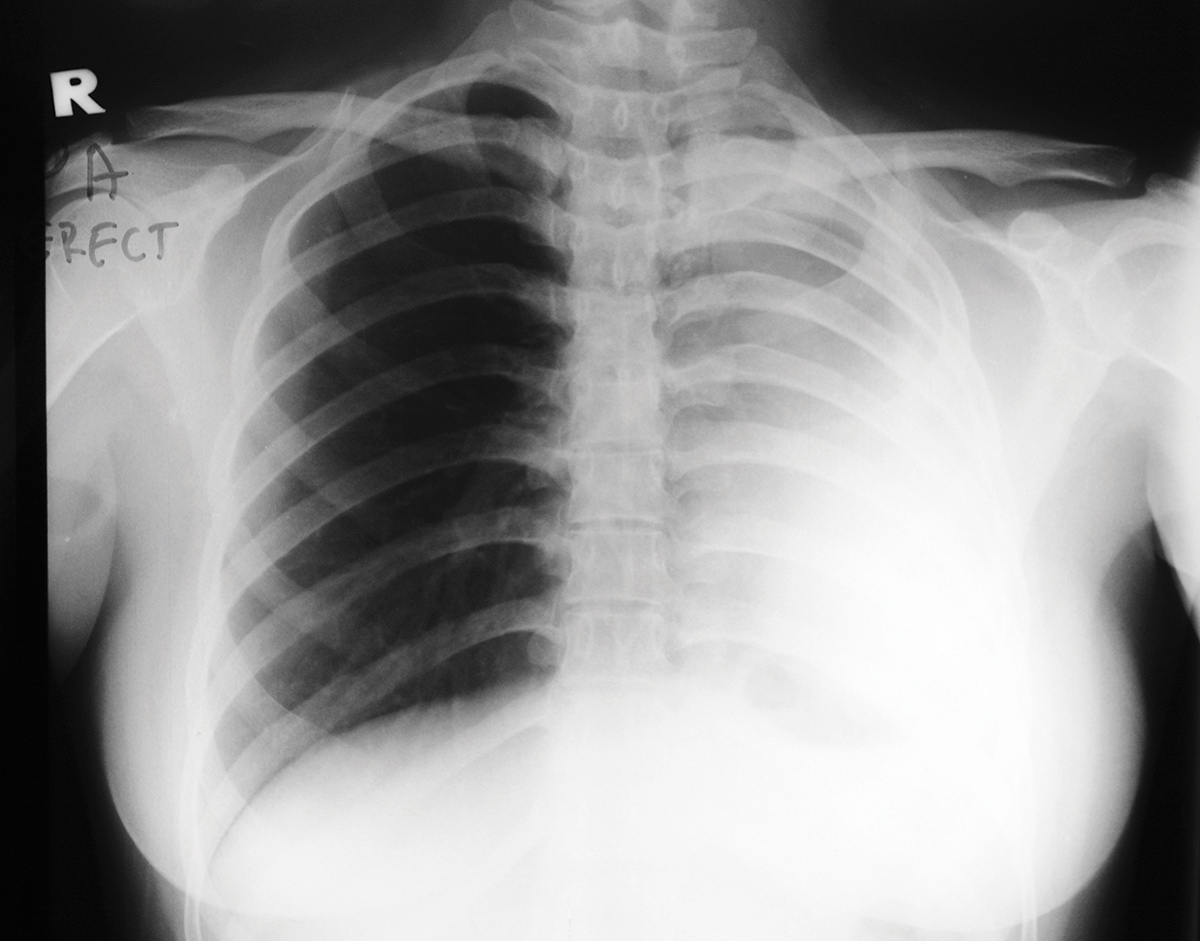
\includegraphics[width=0.6\textwidth,keepaspectratio=true]{lung_opacity}
	\caption{
		RTG z objawami zwłóknienia. Widać małe okrągłe formacje z efektem mlecznej szyby
	}
\end{figure}

%-----------------------------------------------------------------------------------
\subsection{Zapalenie płuc}
Zapaleniem płuc nazywamy stan zapalny przy którym są zapalone pęcherzyki płucne. Przyczyną choroby są zwykle infekcje wirusowe lub bakteryjne. Objawami tej choroby zwykle są gorączka, kaszel, ból w klatce piersiowej, trudność w oddychaniu. Jedną z metod diagnostyki i najbardziej popularną jest metoda robienia zdjęć rentgenowskich. RTG jest narzędziem które pomaga lekarzom diagnozować zapalenie płuc. Na RTG zapalenie widać jako jasny obszar.

\begin{figure}[H]
	\centering
	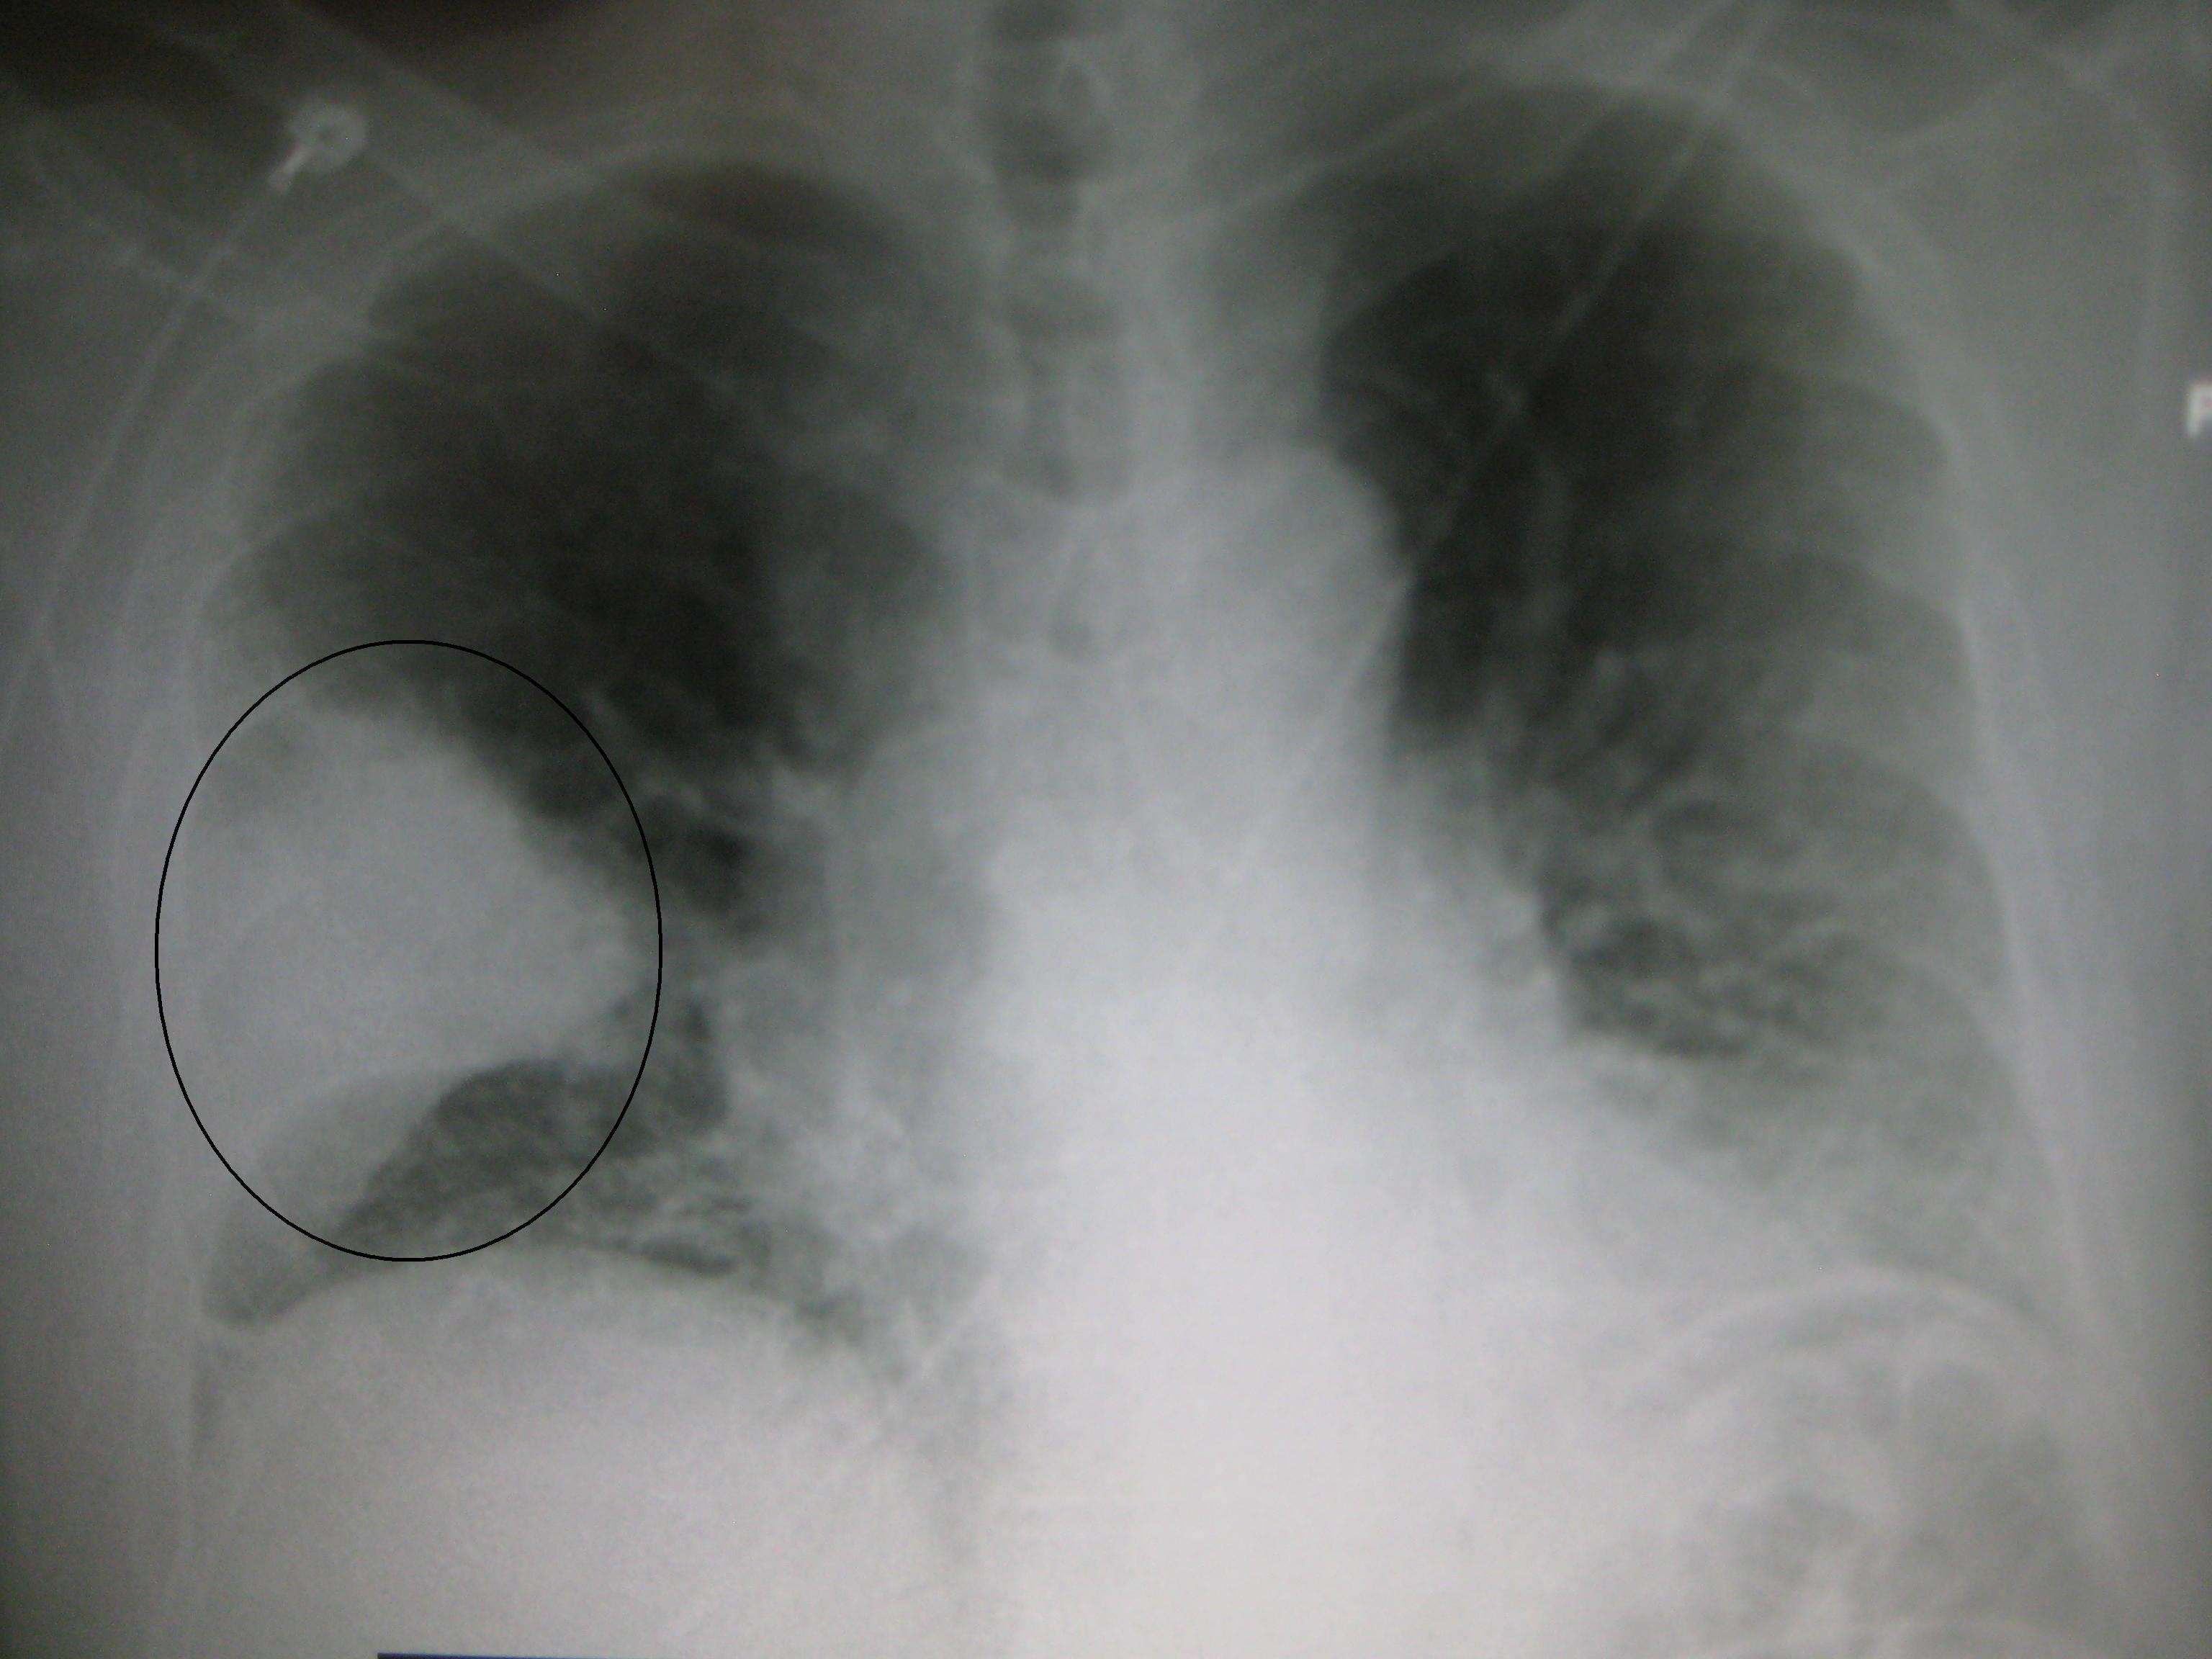
\includegraphics[width=0.6\textwidth,,keepaspectratio=true]{viral_pneumopnia}
	\caption{
		RTG z ostrą formą zapalenia płuc. Obszar z zapaleniem jest jasny i pokazany na rysunku czarnym kołem.
	}
\end{figure}

%-----------------------------------------------------------------------------------
\subsection{COVID-19}
COVID-19 (od ang. \textit{coronavirus disease 2019}) – jest to choroba spowodowana zakażeniem wirusem SARS-CoV-2. Covid może powodować jak efekt mlecznej szyby tak i zapalenie płuc. Metodami diagnozowania są zwykle różnego rodu sprawdzenia krwi na przeciwciała, łańcuchowej reakcji polimerazy oraz komputerowej tomografii. Czasem do diagnozowania przydaje się RTG.

\begin{figure}[H]
	\centering
	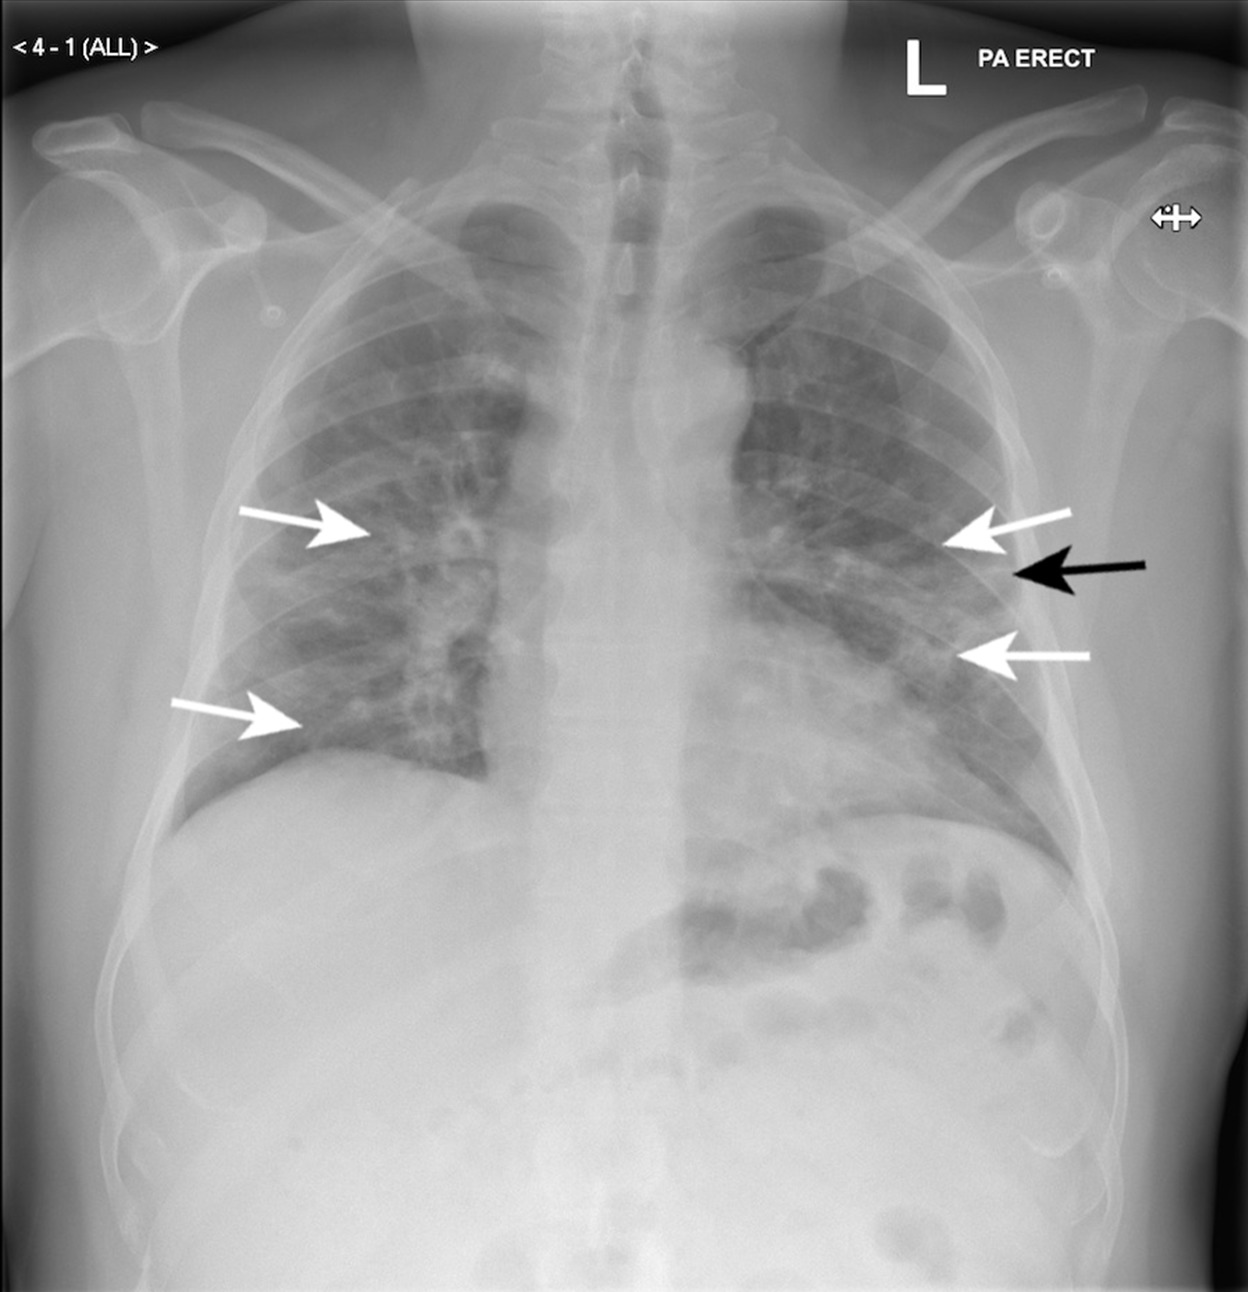
\includegraphics[width=0.6\textwidth,keepaspectratio=true]{covid}
	\caption{
		COVID-19
	}
\end{figure}

%===================================================================================
\section{Uczenie maszynowe}
Uczeniem maszynowym nazywa się dziedzina nauki programowania komputerów w sposób umożliwiający im uczenie się z danych \cite{geron} 
Ta praca jest zrobiona z użyciem uczenia maszynowego a zwłaszcza sieci neuronowych.


%===================================================================================
\section{Neuron}
Zanim opiszę sieci neuronowe, chcę przedstawić co to jest neuron (komórka).

\subsection{Neuron biologiczny}
%??PLAGIAT?? Różne żródła
Jak wiadomo mózg ludzki i większości innych organizmów składa się z malutkich komórek nerwowych, nazywanych neuron, zdolnych do przetwarzania i przewodzenia informacji w postaci sygnału elektrycznego. Neurony są podstawowym elementem układu nerwowego zwierząt. Najwięcej neuronów znajduje się w ośrodkowym układzie nerwowym, w skład którego wchodzi mózgowie oraz rdzeń kręgowy. \cite{neuroscience}
Głównymi elementami neuronu są ciało komórki zawierające jądro i większość organelli komórkowych, wiele rozgałęziających się wypustek zwanych dendrytami oraz jedna bardzo długa wypustka -- akson. \cite{geron}

\begin{figure}[H]
	\centering
	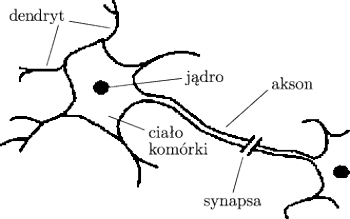
\includegraphics[width=\textwidth,height=6cm,keepaspectratio=true]{neuron_bio}
	\caption{
		Obraz komórki biologicznej \cite{neuron_bio}
	}
\end{figure}

Neurony biologiczne generują krótkie impulsy elektryczne zwane sygnałami, które są przenoszone wzdłuż aksonów i powodują uwalnianie w synapsach sygnałów chemicznych zwanych neuroprzekaźnikami. Kiedy komórka nerwowa otrzymuje dostateczną liczbę neuroprzekaźników od innych neuronów w ciągu kilku milisekund, to sama zaczyna wysyłać własne sygnały elektryczne (w rzeczywistości jest to uzależnione od neuroprzekaźników, gdyż niektóre z nich hamują aktywność komórki nerwowej). \cite{geron}
Zatem mechanizm działania poszczególnych neuronów jest dość prosty, tworzą one jednak rozległą sieć składającą się z miliardów komórek nerwowych, gdzie zazwyczaj jeden neuron łączy się z tysiącami innych. Dzięki tak olbrzymiej sieci zawierającej proste komórki nerwowe mogą być wykonywane skomplikowane obliczenia.

%-----------------------------------------------------------------------------------
\subsection{Sztuczny neuron}
W 1943 przez Warren S. McCulloch i Walter Pitts było zaproponowano bardzo prostą reprezentację neuronu sztucznego. On ma co najmniej jedno binarne wejście i dokładnie jedno binarne wyjście. Wyjście zostanie aktywne tylko wtedy kiedy będzie aktywna określona liczba wejść. \cite{mcculloch1943logical} Tak prosty model daje nam bardzo duże możliwości. Twórcy udowodnili że za pomocą takich neuronów jesteśmy w stanie zaprotestować sieć która rozwiąże dowolne zadanie logiczne.

Frank Rossenblatt trochę zmodyfikował ten neuron.\newline
Kluczowe zmiany:
\begin{itemize}
	\item Wartościami wejść/wyjść są liczby
	\item Każde połączenie ma przyporządkowaną wagę.
	\item Używanie funkcji skokowej na końcu
	\item Dodatkowe obciążeniowe wejście(zawsze wysyła wartość 1) z własną wagą, tak zwany bias
\end{itemize}
Jednostka wylicza ważoną sumę sygnałów wejściowych, a następnie zostaję użyta funkcja aktywacji. Najczęściej zostaje użyta funkcja skokowa Heaviside`a (Rysunek \ref{Heaviside}) lub signum (Rysunek \ref{Signum}) .Przy użyciu skokowej funkcji aktywacji taki neuron można nazywać progową jednostką logiczną lub liniową jednostką progową (ang. \textit{Linear Treshod Unit} -- LTU). Działanie tej jednostki można matematycznie opisać w następujący sposób.\newline\newline
$ y = \mathcal{H}(W^{T}X + b) $\newline \newline
Gdzie: \newline
X -- wektor wejść. \newline
W -- wektor wag. \newline
b -- bias. \newline
y -- wyjście neuronu. \newline
$ \mathcal{H}(...) $ -- funkcja skokowa Heaviside`a\newline

\begin{figure}[H]
	\centering
	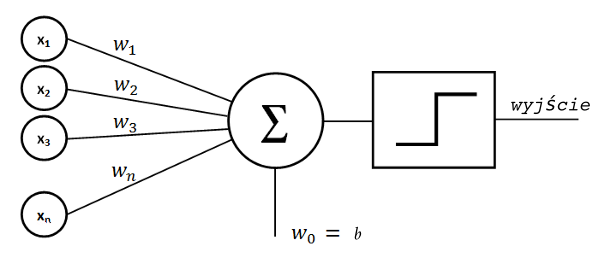
\includegraphics[width=0.8\textwidth,keepaspectratio=true]{neuron_rosenblatta}
	\captionof{figure}{
		Sztuczny neuron Franka Rosenblatta
	}
\end{figure}

%===================================================================================
\section{Funkcji użyte w pracy}

%-----------------------------------------------------------------------------------
\subsection{Funkcja skokowa Heaviside’a}
Funkcja skokowa Heaviside’a, skok jednostkowy – funkcja nieciągła, która przyjmuje wartość dla ujemnych argumentów i wartość 1 w pozostałych przypadkach:

\begin{equation}
	\mathcal{H}(x) = 
	\begin{cases}
		0 & \text{dla $x < 0$}\\
		1 & \text{dla $x \geqslant 0$ }\\
	\end{cases}    
\end{equation}

\begin{figure}[H]
	\centering
	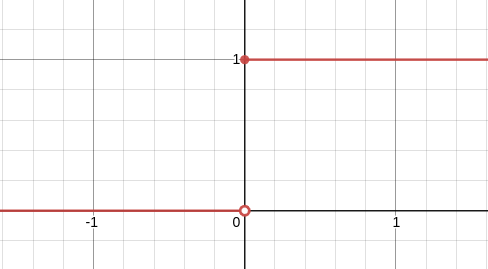
\includegraphics[width=0.6\textwidth,keepaspectratio=true]{Heaviside}
	\caption{
		Funkcja skokowa Heaviside’a
	}
	\label{Heaviside}
\end{figure}


%-----------------------------------------------------------------------------------
\subsection{Signum}
Signum, sgn (łac. signum „znak”) – funkcja zmiennej rzeczywistej, zdefiniowana następująco:
\begin{equation}
	sgn(x) = 
	\begin{cases}
		-1 & \text{dla $x < 0$}\\
		0 & \text{dla $x = 0$}\\
		1 & \text{dla $x > 0$}\\
	\end{cases}    
\end{equation}

\begin{figure}[H]
	\centering
	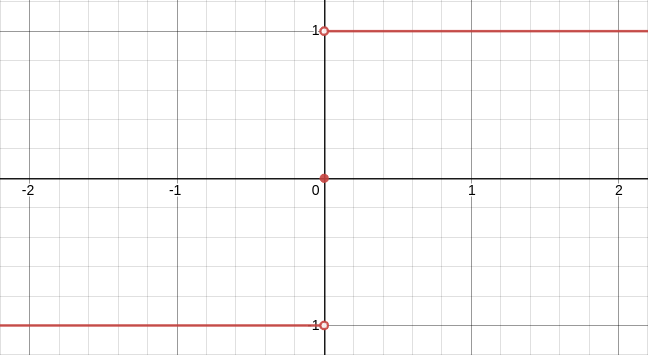
\includegraphics[width=0.6\textwidth,keepaspectratio=true]{Signum}
	\caption{
		Signum
	}
	\label{Signum}
\end{figure}


%-----------------------------------------------------------------------------------
\subsection{Sigmoid}
Funkcja sigmoidalna jest funkcją matematyczną mającą charakterystyczną krzywą w kształcie litery „S” lub krzywą sigmoidalną.
Typowym przykładem funkcji sigmoidalnej jest funkcja logistyczna pokazana na rysunku \ref{Sigmoid} i zdefiniowana wzorem: 


\begin{figure}[H]
	\begin{center}
		$S(x) = \dfrac{1}{1 + e^{-x}}$
	\end{center}
	
	\centering
	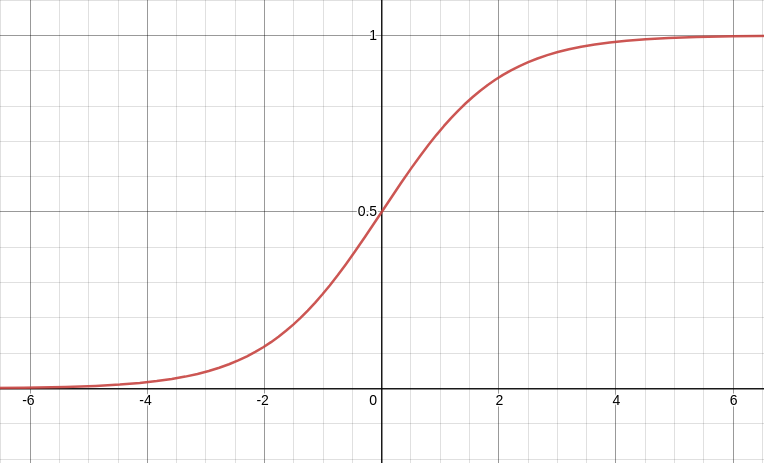
\includegraphics[width=0.6\textwidth,keepaspectratio=true]{Sigmoid}
	\caption{
		Sigmoid
	}
	\label{Sigmoid}
\end{figure}

%-----------------------------------------------------------------------------------
\subsection{ReLU}
Kolejną, popularną funkcją aktywacji jest ReLU (rectifier Linear Unit). Od swojego kształtu w mowie potocznej często nazywana jest funkcją rampy (bo i rzeczywiście - wygląda jak rampa).
\begin{equation}
	ReLU(x) = 
	\begin{cases}
		0 & \text{dla $x < 0$}\\
		x & \text{dla $x \geqslant 0$ }\\
	\end{cases}    
\end{equation}

\begin{figure}[H]
	\centering
	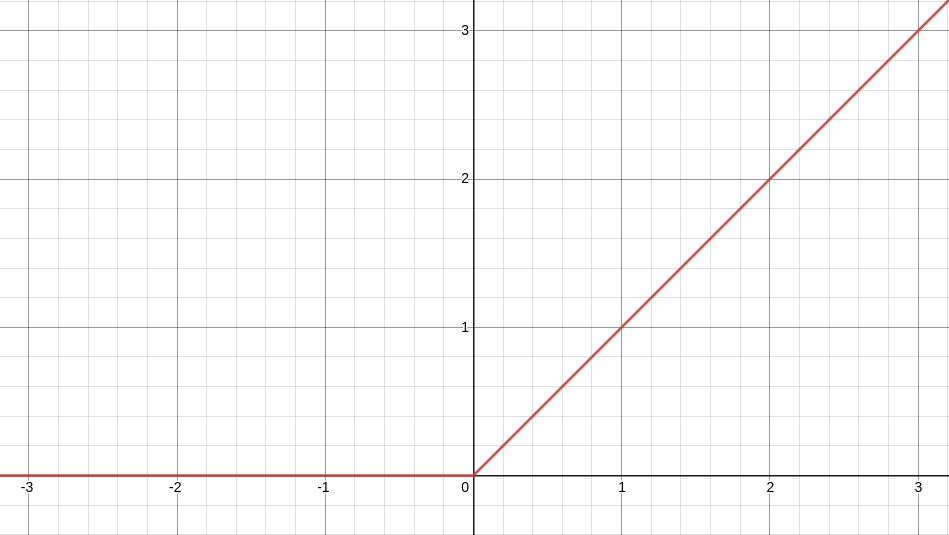
\includegraphics[width=0.6\textwidth,keepaspectratio=true]{ReLu}
	\caption{
		ReLU
	}
\end{figure}

%-----------------------------------------------------------------------------------
\subsection{Softmax}
Funkcja softmax przyjmuje jako dane wejściowe wektor z $K$ liczb rzeczywistych i normalizuje go do rozkładu prawdopodobieństwa składającego się z $K$ prawdopodobieństw proporcjonalnych do wykładników liczb wejściowych. Oznacza to, że przed zastosowaniem softmaxa niektóre składowe wektora mogą być ujemne lub większe niż jeden; i może nie sumować się do 1; ale po zastosowaniu softmaxu każdy składnik będzie w przedziale $[0,1]$, a składniki będą sumować się do 1, aby można je było interpretować jako prawdopodobieństwa. Co więcej, większe komponenty wejściowe będą odpowiadać większym prawdopodobieństwu.

\begin{center}
	\begin{equation}	
		z = Softmax(t) = \mathcal{S}(t) = \dfrac{e^{t_i}}{\sum_{j=1}^{K}e^{t_j}}\text{\quad dla i = ,...,K.}
		\label{softmax}
	\end{equation}
	\ref{softmax}: Obliczanie Softmax
\end{center} 

\begin{flushleft}
	Gdzie:\newline
	K -- ilość neuronów warstwy wyjściowej\newline
	t -- wektor wyjść
	
\end{flushleft}

%-----------------------------------------------------------------------------------
\subsection{Entropia krzyżowa, Cross-Entropy}
Entropia krzyżowa jest to funkcja kosztu. Oznacza odległość między dwoma rozkładami prawdopodobieństw.

\begin{center}
	\begin{equation}	
		CE(z, y) = -\sum_{i=1}^{K}y_i \log z_i
		\label{CrossEntropy}
	\end{equation}
	\ref{CrossEntropy}: Obliczanie entropii krzyżowej
\end{center} 

\begin{flushleft}
	Gdzie:\newline
	$z$, $y$ -- rozkłady prawdopodobieństw
\end{flushleft}

%===================================================================================
\section{Sieć neuronowa}
Sieć neuronowa to połączenie neuronów w jakiś sposób. Najbardziej popularne są sieci całkowicie powiązane, jednokierunkowe (ang. \textit{feedforward, fully connected})

\begin{figure}[H]
	\centering
	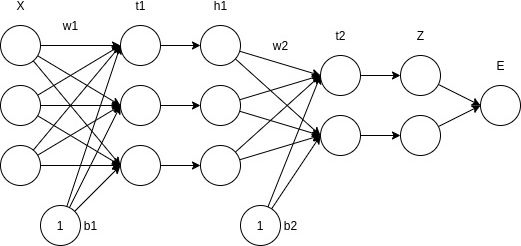
\includegraphics[width=0.6\textwidth,keepaspectratio=true]{feed_forward_network}
	\caption{
		Sieć neuronowa  
	}
	\label{feed_forward_network}
\end{figure}

Na rysunku \ref{feed_forward_network} jest pokazana sieć neuronowa składająca się z trzech warstw: jednej warstwy wejściowej, jednej wyjściowej i jednej ukrytej. Dla ułatwienia obliczeń wektorów wyjść ukrytej i wyjściowej warstwy, obliczania są podzielone na dwie fazy: nieliniową $X \rightarrow t_1; h_1 \rightarrow t_2$ i liniową $t_1 \rightarrow h_1; t_2 \rightarrow z$.

\begin{flushleft}
	$X$ -- wektor wejść (pierwszej warstwy) \newline
	$W_1, W_2$ -- matrycy wag drugiej i trzeciej warstw \newline
	$b_1, b_2$ -- wektory wag biasów drugiej i trzeciej warstw \newline
	$t_1, t_2$ -- liniowe wyjścia drugiej i trzeciej warstw w postaci wektorów\newline
	$h_1$ -- nieliniowe wyjście drugiej warstwy, wektor \newline
	$z$ -- wektor wyjść Softmax \newline
	$E$ -- skalar błędu
\end{flushleft}

\begin{figure}[H]
	\centering
	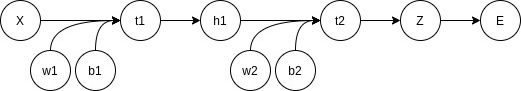
\includegraphics[width=0.6\textwidth,keepaspectratio=true]{feed_forward_graph}
	\caption{
		Graf obliczenia wyjścia sieci i błędu  
	}
	\label{feed_forward_graph}
\end{figure}


Obliczamy wszystko po kolei. Jest sprawą dość prostą. Dla obliczenia wektora wyjścia z każdej warstwy sieci potrzebujemy mieć matrycy wag i wektory biasów. Najcięższej one są inicjalizowane losowo

\begin{flushleft}
Dla obliczenia pierwszej fazy pierwszej warstwy potrzebne są matryca wag i wektor biasów tej warstwy. Wektor wejść tej warstwy mnożymy przez matryce wag i dodajemy wektor biasów.\\
$t_1 = XW_1 + b_1;$\\

Dla obliczenia drugiej fazy(nieliniowej) poprzedni rezultat przeprowadzamy przez funkcje aktywacji.\\
$h_1 = F(t_1);$\\

Metoda obliczania każdej następnej warstwy sieci neuronowej (obliczanie wektorów, czasami matryc lub tensorów. To zależy od wymiarowości danych treningowych) jest dokładnie taka sama. Wektor wejść tej warstwy mnożymy przez matryce wag i dodajemy wektor biasów.\\
$t_2 = h_1W_2 + b_2;$\\

Ostatnia warstwa zwykle ma Softmax jako funkcje aktywacji.\\
$z = \mathcal{S}(t_2);$\\

Dla otrzymania skalaru błędu jest wykorzystana metoda entropii krzyżowej.\\
$E = CE(z,y);$

\end{flushleft}


%===================================================================================
\section{Nadzorowane uczenie sztucznych sieci neuronowych}
Proces uczenia sieci polega na tym że zmieniamy wagi neuronów i biasów w sposób który prowadzi do zmniejszenia błędu na wyjściu sieci. Zmierzyć ten błąd nie jest trudno, wyżej to już zostało opisane. Uczenie składa się z dwóch etapów: etapu obliczenia gradientu i etapu optymizacji wag. 
Dla pierwszego etapu w swojej prace używam algorytmu propagacji wstecznej (ang. \textit{back propagation}). Natomiast dla etapu optymizacji używam optymizatora Adaptive Moment Estimation (Adam)

%===================================================================================
\section{Propagacja wsteczna}
%PLAGIAT
Algorytm propagacji wstecznej stanowi dzisiaj podstawowy algorytm uczenia nadzorowanego wielowarstwowych jednokierunkowych sieci neuronowych. Podaje on przepis na zmianę wag w dowolnych połączeń elementów przetwarzających rozmieszczonych w sąsiednich warstwach sieci jednokierunkowej. Jest to algorytm oparty na minimalizacji sumy kwadratów błędów uczenia. Dzięki zastosowaniu specyficznego sposobu propagowania błędów uczenia sieci powstałych na jej wyjściu, tzn. przesyłania ich od warstwy wyjściowej do wejściowej, algorytm propagacji wstecznej stał się jednym z najskuteczniejszych algorytmów uczenia sieci. \cite{nn_jozef}

%-----------------------------------------------------------------------------------
\subsection{Znależenie gradientu ostatniej warstwy}
\begin{figure}[H]
	\centering
	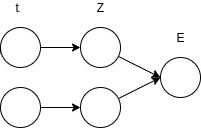
\includegraphics[width=0.3\textwidth,keepaspectratio=true]{feed_forward_error}
	\caption{Osobno narysowana ostatnia warstwa sieci na rysunku \ref{feed_forward_network}}
	\label{feed_forward_error}
\end{figure}

Wyliczanie wyjścia Softmax\\
$z = Softamx(t) = \mathcal{S}(t)= \frac{e^{t_i}}{\sum_{j=1}e^{t_i}}$ \\

Do wyliczania skalaru błędu potrzebujemy $z$ - wektor wyjść sieci oraz $y$ - wektor poprawnej odpowiedzi w postaci wektora z taką samą wymiarowością jak i wektor wyjścia sieci.\\
$E = CrossEntropy(z, y) = -\sum_{i=1}y_i\log z_i$\\

W tym przypadku błąd jest wyliczany w ten sposób, z użyciem formuły Softmax\\
$E = CE(\mathcal{S}(t),y)=-\sum_{i=1}y_i\log\frac{e^{t_i}}{\sum_{j=1}e^{t_i}}$\\
$= -\sum_{i=1}y_i(t_i-\log \sum_{j=1}e^{t_i}) =$\\
$= -\sum_{i=1}y_it_i + \sum_{i=1}y_i\log\sum_{j=1}e^{t_i} =$\\
$= -\sum_{i=1}y_it_i + \log\sum_{j=1}e^{t_i}$\\
Po nietrudnych przekształceniach otrzymujemy powyższą formułę.\\

Do propagacji wstecznej jest potrzebna pochodna błędu. Można bardzo łatwo ją policzyć dla poszczególnego neuronu $t_k$ -- k-ty neuron warstwy $t$ \\
$\frac{\delta E}{\delta t_k} = -y_k + \frac{1}{\sum_{j=1}e^{t_j}}\cdot e^{t_k} = \mathcal{S}_k - y_k$\\

Można zauważyć że otrzymaliśmy wzór na Softmax. Czyli pochodną błędu po wyjściu warstwy t można bardzo łatwo policzyć, po prostu, od wektora wyjść sieci odjąć wektor oczekiwany.\\ 
$\frac{\delta E}{\delta t} = \mathcal{S}(t) - y = z - y$

\begin{figure}[H]
	\centering
	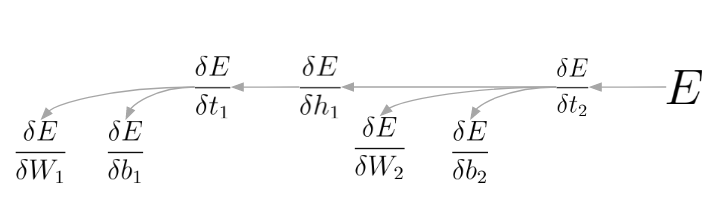
\includegraphics[width=0.6\textwidth,keepaspectratio=true]{gradient_graph}
	\caption{Graf obliczenia gradientu}
	\label{gradien_graph}
\end{figure}

\begin{flushleft}
Obrachunki otrzymania reszty pochodnych:\\
$\dfrac{\delta E}{\delta t_2} = S(t_2)-y=z-y$\\
\vspace{5mm}
$\dfrac{\delta E}{\delta W_2} = h_1^T \cdot \dfrac{\delta E}{\delta t_2}$\\
$\dfrac{\delta E}{\delta b_2} = \dfrac{\delta E}{\delta t_2}$\\
\vspace{5mm}
$\dfrac{\delta E}{\delta h_1} = \dfrac{\delta E}{\delta t_2} \cdot W_2^T$\\
$\dfrac{\delta E}{\delta t_1} = \dfrac{\delta E}{\delta h_1} \odot F^\prime (t_1)$\\
\vspace{5mm}
$\dfrac{\delta E}{\delta W_1} = X^T \cdot \dfrac{\delta E}{\delta t_1}$\\
$\dfrac{\delta E}{\delta b_1} = \dfrac{\delta E}{\delta t_1}$
\end{flushleft}

%===================================================================================
\section{Splotowe sieci neuronowe}
Jak wiadomo do wizji komputerowej już od dawna używają sieci neuronowe. Ale jeśli używać do tego zwykłych neuronów powiązanych w sieci feedforward, fully connected, to będziemy mieli za dużo wag. Przypuśćmy że mamy kolorowy obrazek 200x200 pikseli. Ilość pikseli będzie 200*200*3=120000. Już mamy bardzo dużo neuronów przecież to tylko warstwa wejściowa, Jeżeli następna warstwa będzie miała 512 neuronów (co jest rzeczywiście za mało), to w pierwszej warstwie będzie 61440000 wag. Jest to bardzo dużo. 
Splotowe sieci, wymyśłone w latach 80 ubiegłego wieku, mogą ulepszyć sytuacje.

%-----------------------------------------------------------------------------------
\subsection{Struktura kory wzrokowej}
%PLAGIAT
David H. Hubel i Torsten Wiesel przeprowadzili szereg eksperymentów na kotach w latach 1958 \cite{David_1958} i 1959 \cite{David_1959}, dzięki którym poznaliśmy strukturę kory wzrokowej. Udowodnili oni w szczególności, że wiele neuronów składających się na korę wzrokową wyznacza lokalne pola recepcyjne, tzn. że reagują jedynie na bodźce wzrokowe mieszczące się w określonym rejonie pola wzrokowego (Rysunek \ref{kora_wzrokowa}). Pola recepcyjne poszczególnych neuronów mogą się na siebie nakładać i łącznie tworzą cale pole wzrokowe \cite{geron}

Do tego badacze pokazali także, że pewne neurony reagują wyłącznie na obrazy składające się z linii poziomych, a inne są pobudzane przez linie ułożone w inny sposób (dwa neurony mogą mieć to samo pole recepcyjne, ale reagować na inne ułożenie linii). Zauważono także, że niektóre komórki nerwowe mają większe pola recepcyjne i wykrywają bardziej skomplikowane kształty, stanowiące połączenie bardziej ogólnych wzorów. Poczynione obserwacje doprowadziły badaczy do wniosku, że neurony odpowiedzialne za rozpoznawanie bardziej skomplikowanych kształtów znajdują się na wyjściu sąsiadujących neuronów reagujących na prostsze bodźce wzrokowe (na rysunku \ref{kora_wzrokowa} każdy neuron jest połączony tylko z kilkoma neuronami z niższej warstwy). Taka archi tektura pozwala wykrywać wszelkie rodzaje skomplikowanych kształtów w obszarze pola wzrokowego. \cite{geron}

\begin{figure}[H]
	\centering
	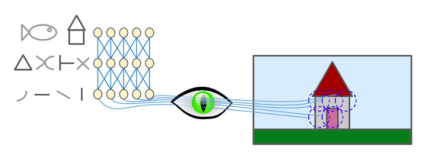
\includegraphics[width=0.6\textwidth,keepaspectratio=true]{kora_wzrokowa}
	\caption{Działanie kory wzrokowej \cite{geron}}
	\label{kora_wzrokowa}
\end{figure}

%-----------------------------------------------------------------------------------
\subsection{Warstwy splotowe}
%PLAGIAT
Najistotniejszym składnikiem sieci CNN jest warstwa splotowa (konwolucyjna): neurony w pierwszej warstwie splotowej nie są połączone z każdym pikselem obrazu wejściowego, lecz wyłącznie z pikselami znajdującymi się w ich polu recepcyjnym (rysunek \ref{warstwa_splotowa}). Z kolei każdy neuron w drugiej warstwie splotowej łączy się wyłącznie z neuronami znajdującymi się w niewielkim obszarze pierwszej warstwy. Dzięki temu sieć może koncentrować się na ogólnych cechach w pierwszej warstwie ukrytej, następnie łączyć je w bardziej złożone kształty w drugiej warstwie ukrytej itd. Taka hierarchiczna struktura jest powszechnie spotykana na zdjęciach, co stanowi jedną z przyczyn tak dużej skuteczności sieci CNN w rozpoznawaniu obrazów. \cite{geron}

Do tej pory wszystkie analizowane przez nas wielowarstwowe sieci neuronowe miały warstwy składające się z długich rzędów neuronów, a przed przekazaniem obrazu do sieci musieliśmy go przekształcić do postaci jednowymiarowej. Od teraz każda warstwa będzie dwuwymiarowa, co ułatwi nam obserwowanie związków pomiędzy neuronami a ich danymi wejściowymi. \cite{geron}
\begin{figure}[H]
	\centering
	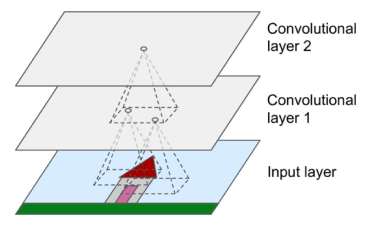
\includegraphics[width=0.6\textwidth,keepaspectratio=true]{warstwa_splotowa}
	\caption{Warstwy CNN \cite{geron}}
	\label{warstwa_splotowa}
\end{figure}

\subsection{Uzupełnianie zerami}
Neuron znajdujący się w wierszu $i$ oraz kolumnie $j$ danej warstwy jest połączony z wyjściami neuronów poprzedniej warstwy zlokalizowanymi w rzędach od $i$ do $i+f_{h}-1$ i kolumnach od $j do j+f_{w}-1$, gdzie $f_{h}$ i $f_{w}$ oznaczają, odpowiednio, wysokość i szerokość pola recepcyjnego (rysunek \ref{padding}). W celu uzyskania takich samych wymiarów każdej warstwy najczęściej są dodawane zera wokół wejść, co zo stało pokazane na rysunku \ref{padding}. Proces ten nazywamy uzupełnianiem zerami (ang. \textit{zero padding}). \cite{geron}
\begin{figure}[H]
	\centering
	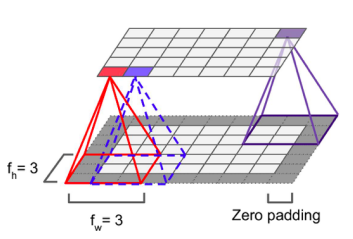
\includegraphics[width=0.6\textwidth,keepaspectratio=true]{padding}
	\caption{Związek pomiędzy warstwami a uzupełnianiem zerami \cite{geron}}
	\label{padding}
\end{figure}

%-----------------------------------------------------------------------------------
\subsection{Krok}
%PLAGIAT
Możliwe jest również łączenie bardzo dużej warstwy wejściowej ze znacznie mniejszą kolejną warstwą poprzez rozdzielanie pól recepcyjnych, tak jak zaprezentowano na rysunku \ref{step}. Rozwiązanie to zmniejsza drastycznie złożoność obliczeniową modelu. Odległość pomiędzy dwoma kolejnymi polami recepcyjnymi nosi nazwę kroku (ang. \textit{stride}). Na widocznym schemacie warstwa wejściowa o wymiarach 5x7 (plus uzupełnianie zerami) łączy się z warstwą o rozmiarze $3 \times 4$ za pomocą pól recepcyjnych będących kwadratami $3 \times 3$ i kroku o wartości 2 (w omawianym przykładzie krok jest taki sam w obydwu wymiarach, ale nie jest to wcale regułą). Neuron zlokalizowany w rzędzie $i$ oraz kolumnie $j$ górnej warstwy łączy się z wyjściami neuronów dolnej warstwy mieszczącymi się w rzędach od $i\times s_{h}$, do $i \times s_{h}+f_{h}-1$ iw kolumnach od $j \times s_{w}$, do $j \times s_{w}+f_{w}-1$. gdzie $s_{h}$ i $s_{w}$, definiują wartości kroków odpowiednio w kolumnach i rzędach. \cite{geron}
\begin{figure}[H]
	\centering
	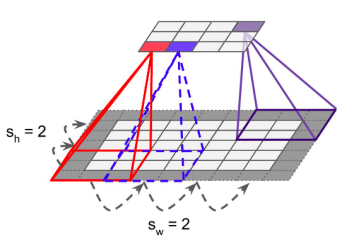
\includegraphics[width=0.6\textwidth,keepaspectratio=true]{step}
	\caption{Redukcja wymiarowości za pomocą kroku o wartość 2 \cite{geron}}
	\label{step}
\end{figure}


%-----------------------------------------------------------------------------------
\subsection{Filtry}
%PLAGIAT
Wagi neuronu mogą być przedstawiane jako niewielki obraz o rozmiarze pola recepcyjnego. Na przykład na rysunku \ref{filters} widzimy dwa możliwe zbiory wag, tak zwane filtry (lub jądra splotowe, ang. \textit{convolution kernels}). Pierwszy filtr jest symbolizowany jako czarny kwadrat z białą pionową linią przechodzącą przez jego środek (jest to macierz o wymiarach $7 \times 7$ wypełniona zerami oprócz środkowej kolumny, która zawiera jedynki); neurony zawierające te wagi będą ignorować wszystkie elementy w polu recepcyjnym oprócz znajdujących się w środkowej pionowej linii (dane wejściowe znajdujące się poza tą linią będą przemnażane przez O). Drugi filtr wygląda podobnie; różnica polega na tym, że środkowa linia jest ułożona poziomo. Także w tym wypadku będą brane pod uwagę jedynie dane wejściowe znajdujące się w tej linii. \cite{geron}

Jeśli wszystkie neurony w danej warstwie będą korzystać z tego samego filtra pionowego" (i takiego samego członu obciążenia), a my wczytamy do sieci obraz zaprezentowany na dole rysunku \ref{filters},to uzyskamy obraz widoczny w lewym górnym rogu rysunku. Po zastosowaniu tego filtru pionowe białe linie stają się wyraźniej widoczne, natomiast pozostała część obrazu zostaje rozmazana. Na zasadzie analogii otrzymujemy obraz widoczny w prawym górnym rogu rysunku po zastosowaniu filtru poziomego"; teraz z kolei białe poziome linie zostają wyostrzone, a reszta obrazu ulega ramazanu. Zatem warstwa wypełniona neuronami wykorzystującymi ten sam filtr daje nam mapę cech (ang. \textit{feature map}), dzięki której możemy dostrzec elementy najbardziej przypominające dany filtr. Nie musisz oczywiście definiować filtrów własnoręcznie - sieć CNN w czasie uczenia wyszukuje filtry najbardziej przydatne do danego zadania i uczy się łączyć je w bardziej złożone
wzorce. \cite{geron}
\begin{figure}[H]
	\centering
	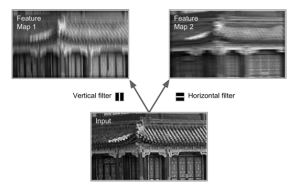
\includegraphics[width=0.8\textwidth,keepaspectratio=true]{filters}
	\caption{Uzyskiwanie map cech za pomocą filtrów \cite{geron}}
	\label{filters}
\end{figure}

%-----------------------------------------------------------------------------------
\subsection{Stosy map cech}
%PLAGIAT
Do tej pory dla uproszczenia przedstawialiśmy każdą warstwę splotową w postaci cienkiej, dwuwymiarowej warstwy, ale w rzeczywistości składa się ona z kilku map cech o identycznych rozmiarach, dlatego trójwymiarowe odwzorowanie jest bliższe rzeczywistości (rysunek \ref{stosy_map_cech}). W zakresie jednej mapy cech każdy neuron jest przydzielony do jednego piksela, a wszystkie tworzące ją neurony współdzielą te same parametry (wagi i człon obciążenia). Neurony w innych mapach cech mają odmienne wartości parametrów. Pole recepcyjne neuronu nie ulega zmianie, ale przebiega przez wszystkie mapy cech poprzednich warstw. Krótko mówiąc, warstwa splotowa równocześnie stosuje różne filtry na wejściach, dzięki czemu jest w stanie wykrywać wiele cech w dowolnym obszarze obrazu \cite{geron}

Dzięki temu, że wszystkie neurony w mapie cech stosują te same parametry, znacznie zmniejsza się ich liczba w modelu, jednak co ważniejsze, oznacza to, że gdy sieć CNN nauczy się rozpoznawać wzorzec w jednym miejscu, będzie w stanie to robić również w innych lokacjach. Dla porównania, sieć GSN po nauczeniu się rozpoznawania wzorca w jednym miejscu nie potrafi tego przełożyć na inne obszary. \cite{geron}

Co więcej, obrazy wejściowe także składają się z kilku warstw podrzędnych, po jednej na każdy kanał barw (ang. \textit{color channel}). Standardowo występują trzy kanały barw - czerwony, zielony i niebieski (ang, red, green, blue-RGB). Obrazy czarno-białe (w odcieniach szarości) zawierają tylko jeden kanał, ale istnieją też takie zdjęcia, które mogą mieć ich znacznie więcej - np. fotografie satelitarne utrwalające dodatkowe częstotliwości fal elektromagnetycznych (takie jak podczerwień). \cite{geron}

W szczególności neuron zlokalizowany w rzędzie $i$ oraz kolumnie $j$ mapy cech $k$ w danej warstwie splotowej $l$ jest połączony z neuronami wcześniejszej warstwy $l-1$ umieszczonymi w rzędach od $i \times s_{h}$ do $i \times s_{h}+f_{h}-1$ i kolumnach od $j \times s_{w}$, do $j \times s+f_{w}-1$ we wszystkich mapach cech (warstwy $l-1$). Zwróć uwagę, że wszystkie neurony znajdujące się w tym samym rzędzie $i$ oraz kolumnie $j$, ale w innych mapach cech są połączone z wyjściami dokładnie tych samych neuronów poprzedniej warstwy. \cite{geron}

Powyższy opis został podsumowany w równaniu \ref{conv_formula} widoczny duży wzór matematyczny służy do obliczania wyniku danego neuronu w warstwie splotowej. Z powodu dużej liczby indeksów równanie to nie wygląda zbyt elegancko, ale za jego pomocą jesteśmy w stanie uzyskać sumę ważoną wszystkich danych wejściowych wraz z członem obciążenia, \cite{geron}

\begin{center}
	\begin{equation}	
		z_{i,j,k}=b_{k}
		\sum_{u=0}^{f_{h}-1}\sum_{v=0}^{f_{w}-1}\sum_{k^\prime=0}^{f_{n^\prime}-1}
		x_{i\prime,j\prime,k\prime}\cdot w_{u,v,k\prime,k}
		\quad gdzie \left\{ \begin{array}{ll}
			i^\prime = i \times s_{h}+u\\
			j^\prime = j\times s_{w}+v
		\end{array} \right.
		\label{conv_formula}
	\end{equation}
	\ref{conv_formula}: Obliczanie wartości wyjściowej neuronu w warstwie splotowej
\end{center}

\begin{figure}[H]
	\centering
	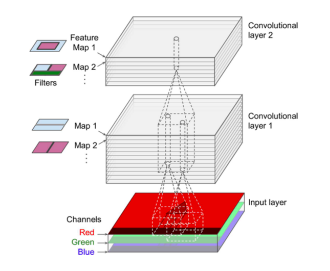
\includegraphics[width=0.6\textwidth,keepaspectratio=true]{stosy_map_cech}
	\caption{Warstwy splotowe zawierające wiele map cech, zdjęcie z trema kanałami barw \cite{geron}}
	\label{stosy_map_cech}
\end{figure}

%-----------------------------------------------------------------------------------
\subsection{Warstwa łącząca (Max pooling)}
%PLAGIAT
Gdy już wiemy, jak działa warstwa splotowa, zrozumienie mechanizmu kryjącego się za warstwami łączącymi (ang. \textit{pooling layers}) nie powinno stanowić problemu. Ich celem jest pod próbkowanie (ang. \textit{subsample}) obrazu wejściowego w celu zredukowania obciążenia obliczeniowego. wykorzystania pamięci i liczby parametrów (a tym samym ograniczenia ryzyka przetrenowania). \cite{geron}

Podobnie jak w przypadku warstw splotowych, każdy neuron stanowiący część warstwy łączącej łączy się z wyjściami określonej liczby neuronów warstwy poprzedniej, mieszczącej się w obszarze niewielkiego, prostokątnego pola recepcyjnego. Podobnie jak wcześniej, musimy tu rozmiar tego pola, wartość kroku, rodzaj uzupełniania zerami itd. Jednakże warstwa licząca nie zawiera żadnych wag; jej jedynym zadaniem jest gromadzenie danych wejściowych za pomocą jakiejś funkcji agregacyjnej, np. maksymalizującej lub uśredniającej. Na rysunku \ref{max_pooling} widzimy najpopularniejszy rodzaj - maksymalizującą warstwę łączącą (ang. \textit{max pooling layer}). W tym przykładzie korzystamy z jądra łączącego (ang. \textit{pooling kernel}) o rozmiarze $2 \times 2$, kroku o wartości 2 iz pominięciem uzupełniania zerami. Jedynie maksymalna wartość z każdego jądra zostaje przekazana do następnej warstwy natomiast pozostałe wartości wejściowe zostają odrzucone. Na przykład w lewym dolnym polu recepcyjnym na rysunku \ref{max_pooling} widzimy wartości wejściowe 1, 5, 3, 2, zatem tylko wartość maksymalna (5) zostanie przekazana do następnej warstwy. Z powodu kroku równego 2 obraz wyjściowy ma szerokość i wysokość o połowę mniejsze w porównaniu do obrazu wejściowego (zaokrąglamy tu w dól. ponieważ nie korzystamy z uzupełniania zerami). \cite{geron}

\begin{figure}[H]
	\centering
	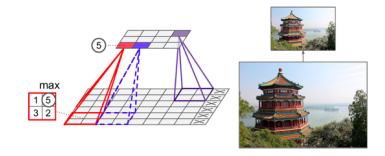
\includegraphics[width=0.8\textwidth,keepaspectratio=true]{max_pooling}
	\caption{Maksymalizująca warstwa łącząca \cite{geron}}
	\label{max_pooling}
\end{figure}


%-----------------------------------------------------------------------------------
\subsection{Warstwa porzucenia (Dropout)}
%PLAGIAT
Najpopularniejszym sposobem do walki z przetrenowaniem w przypadku sieci neuronowych (w tym także konwolucyjne sieci neuronowe) jest porzucanie. Dropout polega na losowym ustawieniu wychodzących krawędzi ukrytych jednostek (neuronów tworzących ukryte warstwy) na 0 przy każdej aktualizacji fazy treningu. Metoda ta jest bardzo efektywna, ponieważ co każde przejście losowo wyłączane są połączenia. Dzięki temu sieć neuronowa nie nauczy się „na pamięć” zbyt szybko, ponieważ architektura co przeliczenie odrobinę się zmienia poprzez zerowanie losowych połączeń neuronów. \cite{jak_dziawaja_cnn}

Po trenowaniu sieci, dropout jest usuwany. Czyli sieć działa normalnie, bez wyłączania połączeń.


%-----------------------------------------------------------------------------------
\subsection{Warstwa spłaszczająca (Flatten)}
%PLAGIAT
Jest to ważny krok. Ta warstwa przekształca naszą wielowymiarową warstwę w sieci w jednowymiarowy wektor. Robimy to po to, aby dopasować dane wejściowe w pełni połączonej warstwy do klasyfikacji. Na przykład tensor o wielkości (10, 10, 3) zostałby przekształcony w wektor o rozmiarze 300 (1, 300). \cite{jak_dziawaja_cnn}

%===================================================================================
\section{Implementacja}
Dla klasyfikacji chorób płuc a głownie COVID-19 zdecydowałem na wykorzystanie splotowej sieci z następnym przejściem w zwykłą sieć jednokierunkową, całkowicie powiązaną. Co w teorii w warstwach splotowych daje możliwość sieci najpierw zauważyć różne kształty, cechy a następnie za pomocą zwykłej sieci neuronowej poprawnie zaklasyfikować chorobę.

%-----------------------------------------------------------------------------------
\subsection{Ostateczna struktura sieci}
Po kilku próbach i eksperymentach ostateczną strukturą sieci jest pięć warstw splotowych które są rozmieszczone na przemian z warstwami łączącymi, na końcu są trzy warstwy zwykłych. Wszystkie warstwy oprócz ostatniej mają funkcje aktywacji ReLU, ostatnia warstwa korzysta z Softmax. Sieć zawiera 16,983,268 parametrów.\\

A dokładniej:
\begin{itemize}
	\item Warstwa wejściowa z wymiarami (299,299,1)
	
	\item Warstwa splotowa. 32 filtry o rozmiarach (5,5)
	\item Warstwa łącząca o rozmiarze (2,2)
	\item Dropout 25\%
	
	\item Warstwa splotowa. 32 filtry o rozmiarach (3,3)
	\item Warstwa łącząca o rozmiarze (2,2)
	\item Dropout 25\%
	
	\item Warstwa splotowa. 64 filtry o rozmiarach (3,3)
	\item Warstwa łącząca o rozmiarze (2,2)
	\item Dropout 25\%
	
	\item Warstwa splotowa. 64 filtry o rozmiarach (3,3)
	\item Warstwa łącząca o rozmiarze (2,2)
	\item Dropout 25\%
	
	\item Warstwa splotowa. 128 filtry o rozmiarach (3,3)
	\item Warstwa łącząca o rozmiarze (2,2)
	\item Dropout 25\%
	
	\item Warstwa spłaszczająca
	\item Dropout 25\%
	
	\item W pełni powiązana warstwa zawierająca 512 neuronów
	\item Dropout 50\%
	
	\item W pełni powiązana warstwa zawierająca 128 neuronów
	\item Dropout 50\%
	
	\item Warstwa wyjściowa zawierająca 4 neurony
\end{itemize}


%-----------------------------------------------------------------------------------
\subsection{Historia uczenia}
\begin{figure}[H]
	\centering
	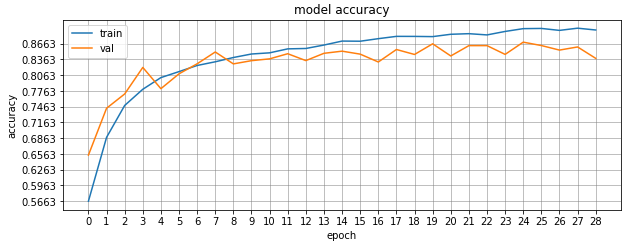
\includegraphics[width=1\textwidth,keepaspectratio=true]{accuracy}
	\caption{}
	\label{accuracy}
\end{figure}

\begin{figure}[H]
	\centering
	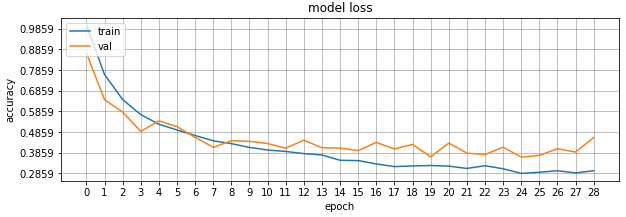
\includegraphics[width=1\textwidth,keepaspectratio=true]{loss}
	\caption{}
	\label{loss}
\end{figure}

Patrząc na wykres historii możemy zobaczyć że przetrenowania wielkiego niema. na końcu rezultat dla danych treningowych jest troszeczkę lepszy co jest całkiem normalną sytuacją. Trochę mnie zdziwiło że na samym początku dane testowe dają lepszy rezultat, to może nam mówić o tym że mamy nie zbyt dobre dane. Najlepszy rezultat był osiągnięty w 24 powtórzeniu. Żeby nie stracić właściwie wytrenowane wagi, po każdej iteracji był robiony backup wag które dają najlepszy rezultat. 
%-----------------------------------------------------------------------------------
\subsection{Stosy map cech}

Żeby lepiej zrozumieć co się dzieje w środku sieci napisałem skrypt który wyświetla mapy cech dla każdej warstwy splotowej.

\begin{figure}[H]
	\centering
	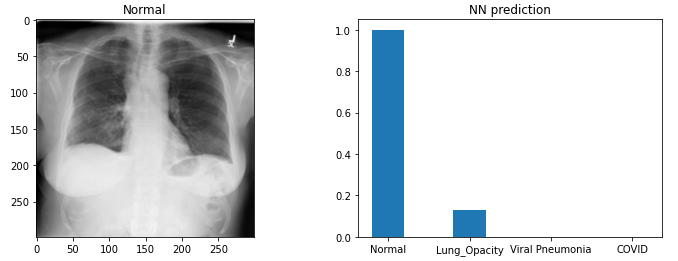
\includegraphics[width=1\textwidth,keepaspectratio=true]{normal_prediction}
	\caption{Predykcja losowego zdjęcia zdrowych płuc ze zbioru testowego.}
	\label{normal_pediction}
\end{figure}

\begin{figure}[H]
\centering
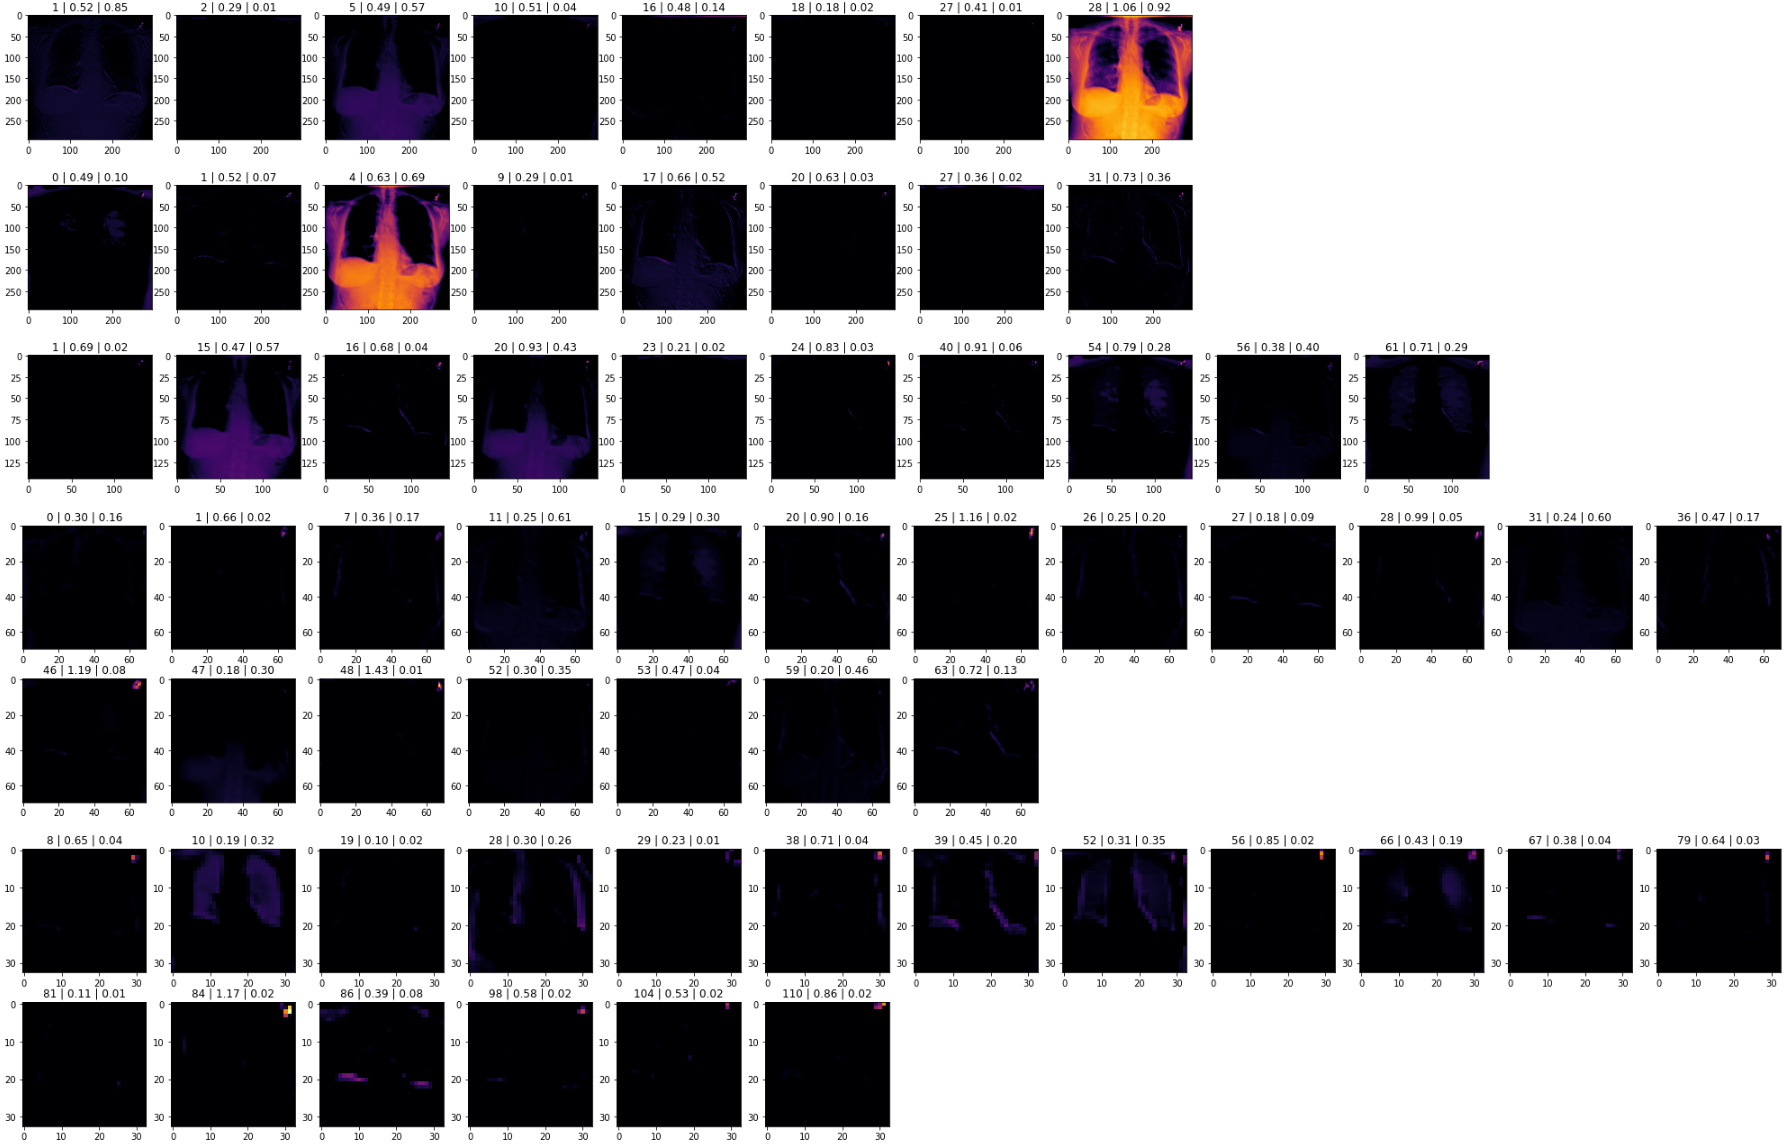
\includegraphics[width=1\textwidth,keepaspectratio=true]{normal_filters_dark}
\caption{Mapy cech generowane pod czas predykcji obrazu na poprzednim rysunku}
\label{normal_filters_dark}
\end{figure}

\begin{figure}[H]
\centering
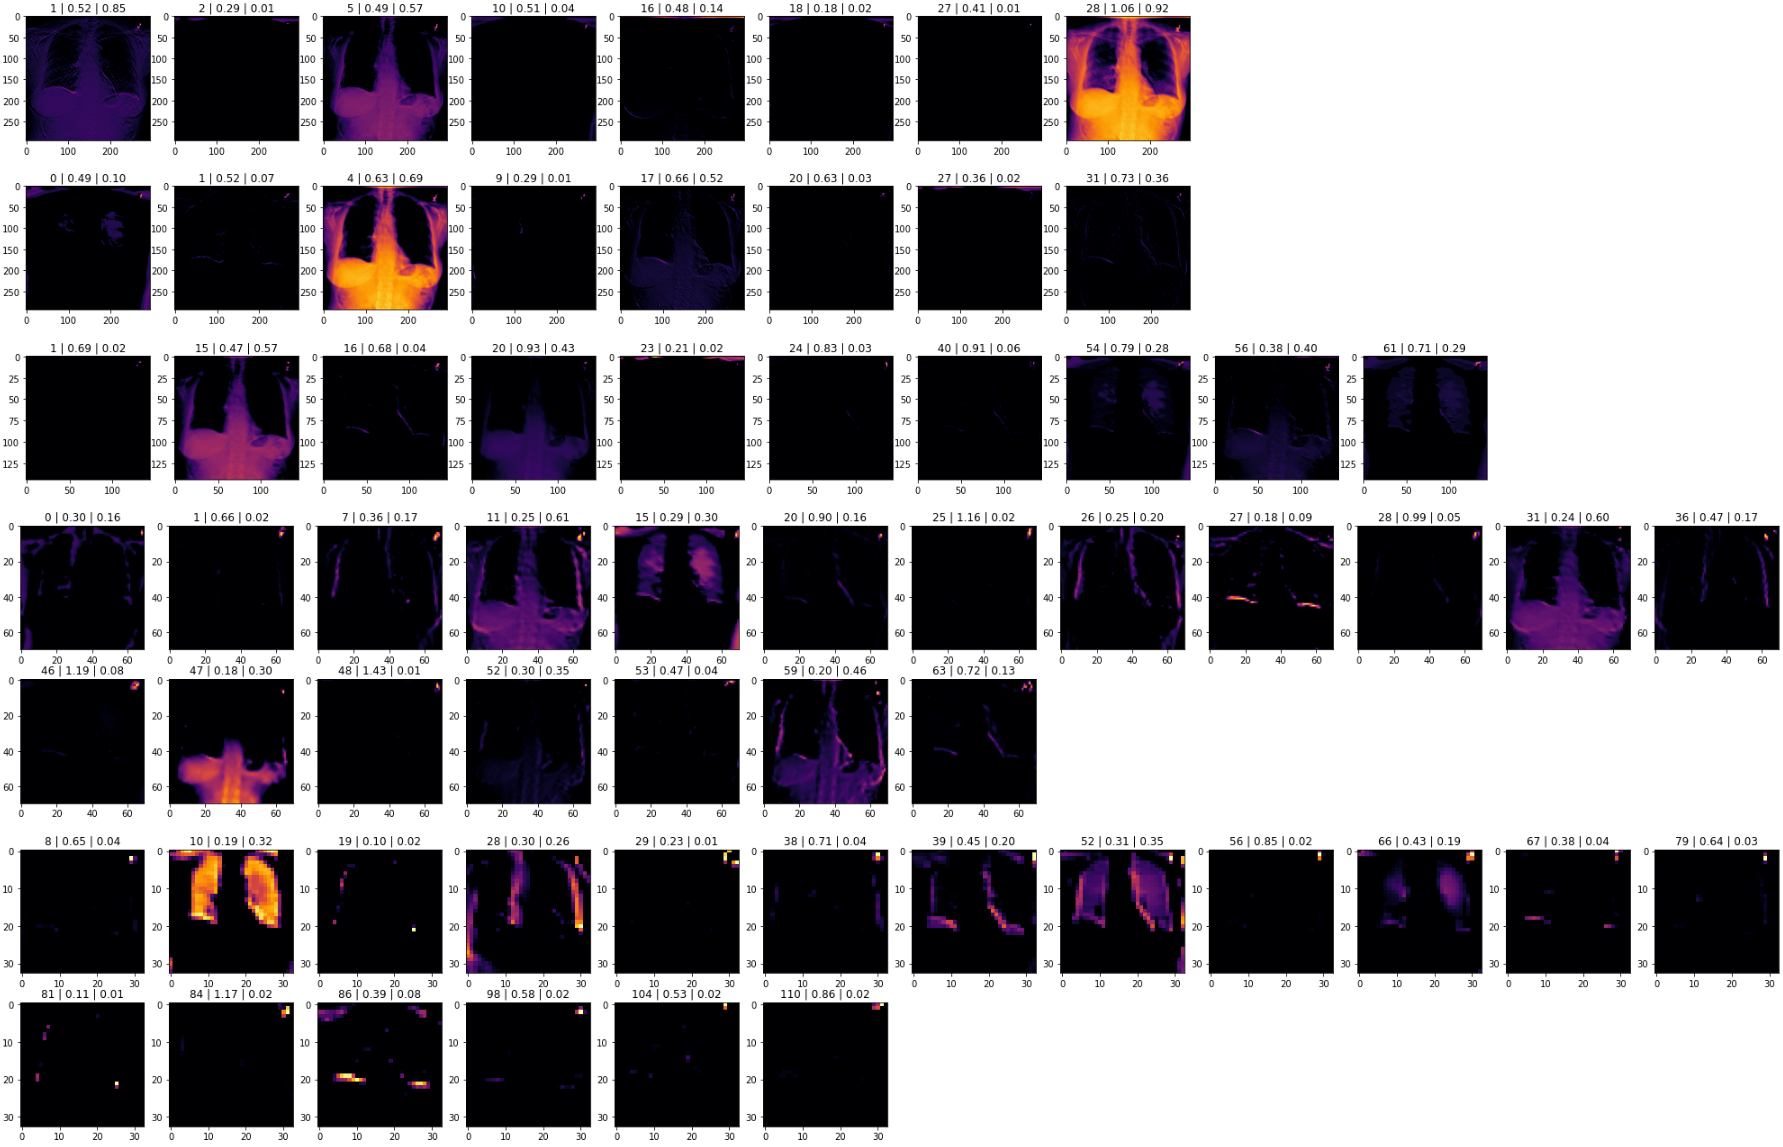
\includegraphics[width=1\textwidth,keepaspectratio=true]{normal_filters_light}
\caption{Bardziej jasne mapy cech generowane pod czas predykcji obrazu na rysunku przed poprzednim}
\label{normal_filters_light}
\end{figure}

Na rysunkach \ref{normal_filters_dark} i \ref{normal_filters_light} są wyświetlone mapy cech generowane przy predykcji choroby płuc na zdjęciu na rysunku \ref{normal_pediction}. Nad każdym obrazkiem są trzy liczby: numer filtry w danej warstwie, maksymalna wartość piksela i procent nie czarnych pikseli na danym obrazku. Są wyświetlone nie wszystkie mapy, dla tego że większość filtrów dają całkowicie czarny obrazek. Różne filtry reagują na różne kształty, dla innych zdjęć są aktywne inne filtry splotowe.

Rysunki \ref{normal_filters_dark} i \ref{normal_filters_light} są identyczne z jedną różnicą, na rysunku \ref{normal_filters_light} obrazki są bardziej jasne, żeby było lepiej widać cechę. Natomiast mapy cech na rysunku \ref{normal_filters_dark} pokazują realną jasność (siłę).

Na rysunku \ref{normal_filters_dark} bardzo dobrze widać że w ostatniej warstwie na obrazku 84 jest najjaśniejszy punkt w prawym górnym kącie. Akurat na zdjęciu w tym miejscu jest odzwierciedlona literka L. Co w teorii mówi nam że ta literka ma wielki wpływ na predykcje choroby. Co w rzeczywistości może być nie tak, dla tego że predykcja jest robiona w następnych warstwach sieci które niestety nie da się tak łatwo wyświetlić i zrozumieć. Natomiast zwiększa to szans że sieć jest wytrenowana źle.  


\begin{figure}[H]
	\centering
	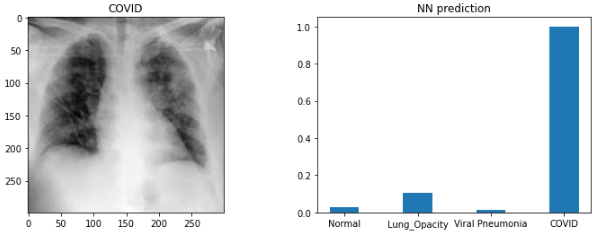
\includegraphics[width=1\textwidth,keepaspectratio=true]{covid_prediction}
	\caption{Predykcja losowego zdjęcia zdrowych płuc ze zbioru testowego.}
	\label{covid_pediction}
\end{figure}

\begin{figure}[H]
	\centering
	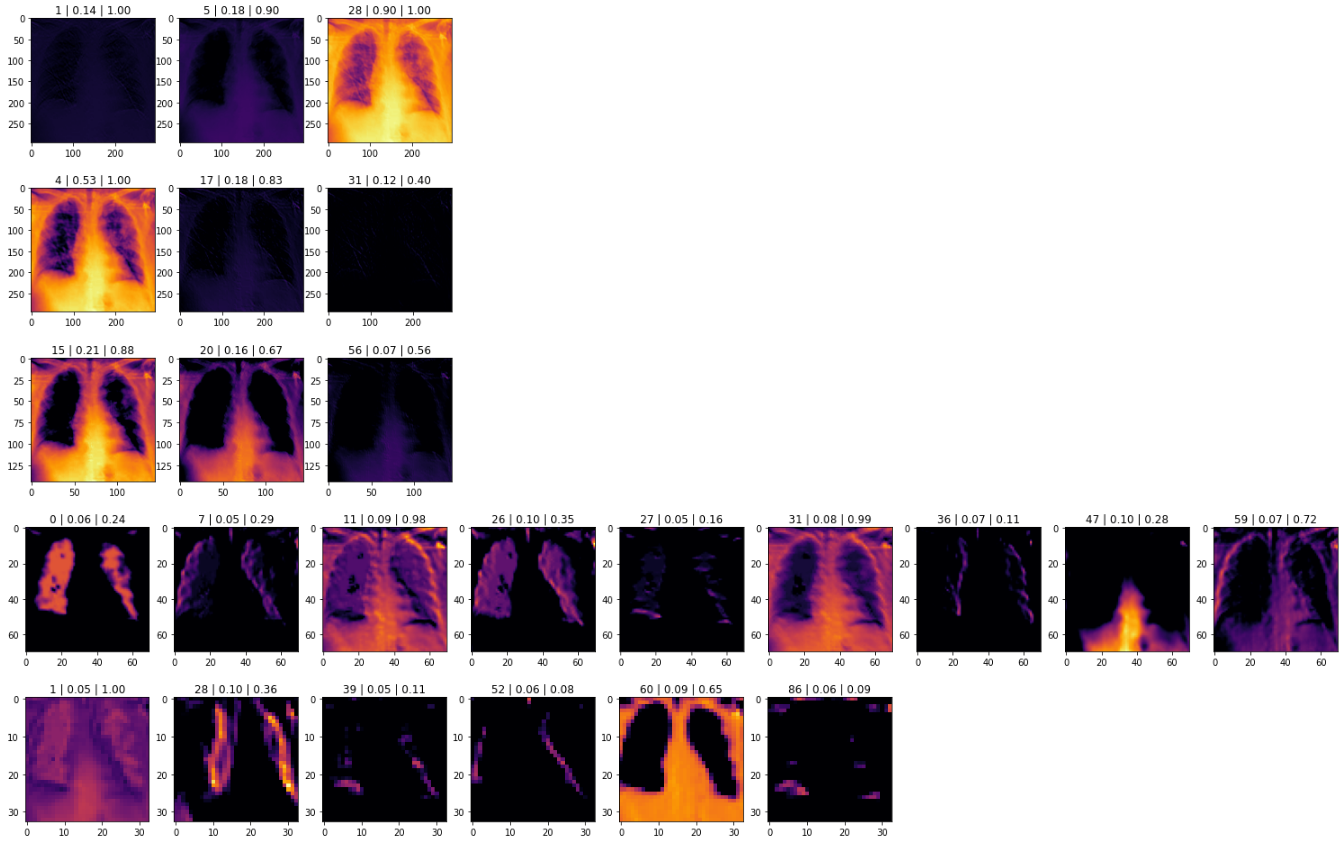
\includegraphics[width=1\textwidth,keepaspectratio=true]{covid_filters_dark}
	\caption{Mapy cech generowane pod czas predykcji obrazu na poprzednim rysunku}
	\label{covid_filters_dark}
\end{figure}

\begin{figure}[H]
	\centering
	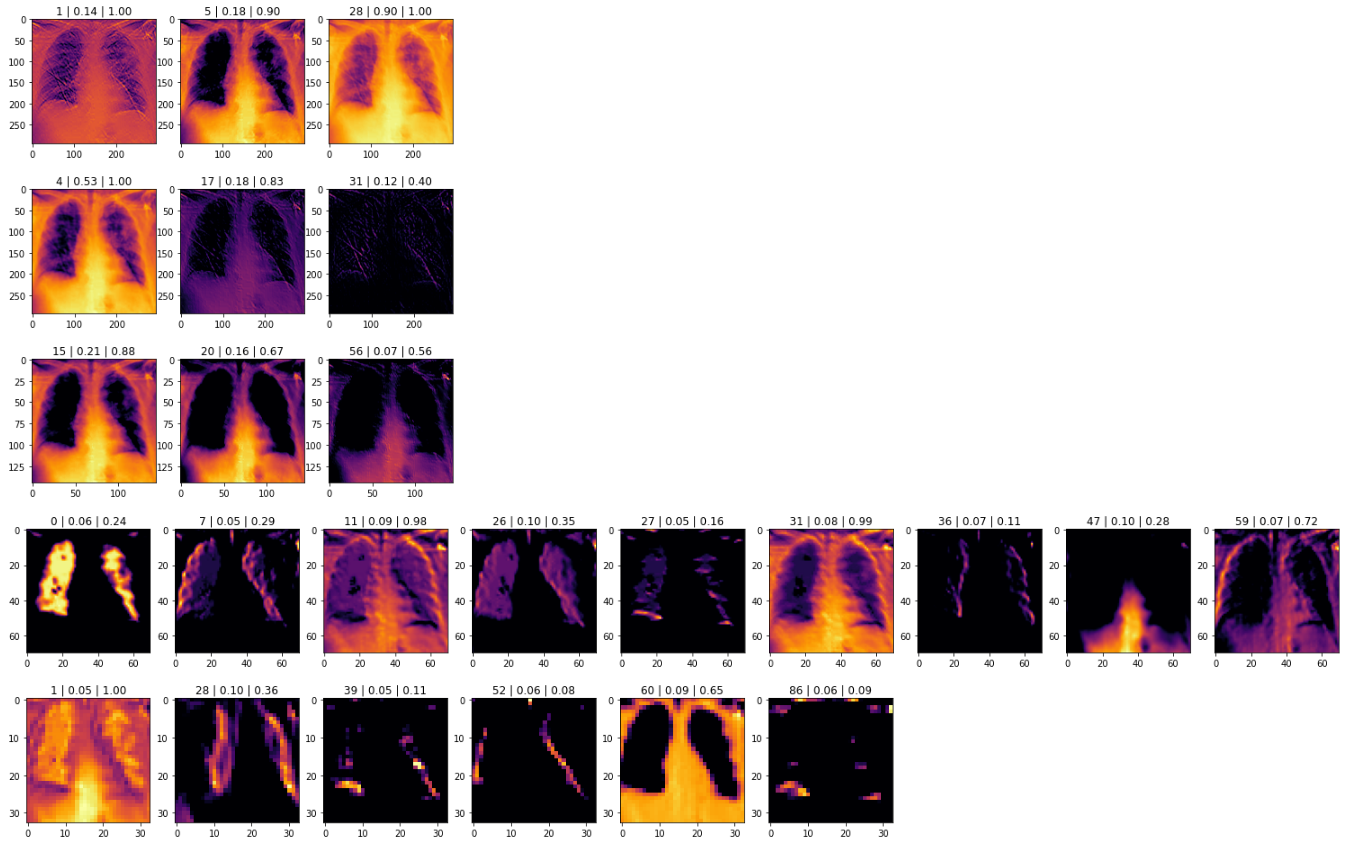
\includegraphics[width=1\textwidth,keepaspectratio=true]{covid_filters_light}
	\caption{Bardziej jasne mapy cech generowane pod czas predykcji obrazu na rysunku przed poprzednim}
	\label{covid_filters_light}
\end{figure}


Na rysunku \ref{covid_pediction} jest pokazana predykcja choroby na zdjęciu bez żadnych literek. Na rysunkach \ref{covid_filters_dark} \ref{covid_filters_light} widać że są aktywne zupełnie inne filtry oraz ilość aktywnych filtrów też jest mniejsza. Na tym przykładzie bardzo dobrze zostały wyróżnione same płuca i różne utwory wewnątrz. Nawet można uwierzyć że sieć coś widzi w płucach i predykcja została zrobiona jakichś utworów wewnątrz. 

%-----------------------------------------------------------------------------------
\subsection{Statystyki używania filtrów splotowych}
Zobaczyłem że dużo filtrów dają czarny obrazek i chciałem sprawdzisz czy na pewno wszystkie filtry reagują na jakieś kształty. Napisałem skrypt który przeprowadził 1000 losowych obrazków ze zbioru testowego przez sieć i policzył średnie wartości otrzymanych map cech. Okazało się że nie wszystkie filtry działają poprawnie. Najprawdopodobniej jest to problem nazywany śmiercią ReLU. W czasie uczenia niektóre neurony trwale "giną", co znaczy, że jedynym przesyłanym sygnałem jest 0. Jeżeli zdarzy się taka sytuacja kiedy wagi neurony zostaną zaktualizowane tak że suma ważona sygnałów wejściowych dla tego neuronu przyjmie wartość ujemną, algorytm optymalizacji wag przestanie  na niego  wpływać ponieważ gradient funkcji ReLU wynosi 0 przy wartościach ujemnych. \cite{geron}

\begin{figure}[H]
	\centering
	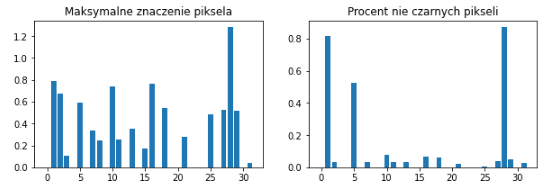
\includegraphics[width=0.8\textwidth,keepaspectratio=true]{statystyka_warstwy_1}
	\caption{Pierwsza warstwa splotowa. Działa 18 filtry z 32}
	\label{statystyka_warstwy_1}
\end{figure}

\begin{figure}[H]
	\centering
	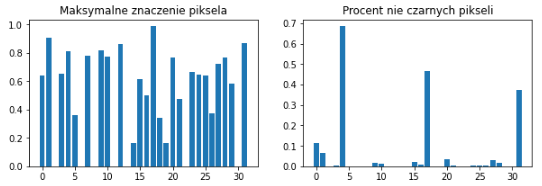
\includegraphics[width=0.8\textwidth,keepaspectratio=true]{statystyka_warstwy_2}
	\caption{Druga warstwa splotowa. Działa 25 filtry z 32}
	\label{statystyka_warstwy_2}
\end{figure}

\begin{figure}[H]
	\centering
	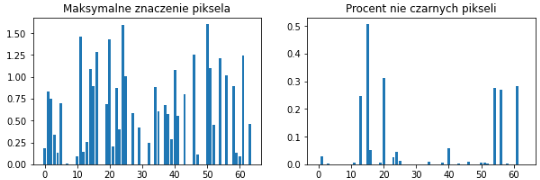
\includegraphics[width=0.8\textwidth,keepaspectratio=true]{statystyka_warstwy_3}
	\caption{Trzecia warstwa splotowa. Działa 44 filtry z 64}
	\label{statystyka_warstwy_3}
\end{figure}

\begin{figure}[H]
	\centering
	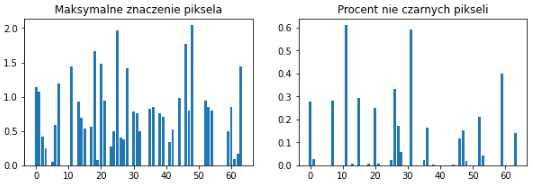
\includegraphics[width=0.8\textwidth,keepaspectratio=true]{statystyka_warstwy_4}
	\caption{Czwarta warstwa splotowa. Działa 43 filtry z 64}
	\label{statystyka_warstwy_4}
\end{figure}

\begin{figure}[H]
	\centering
	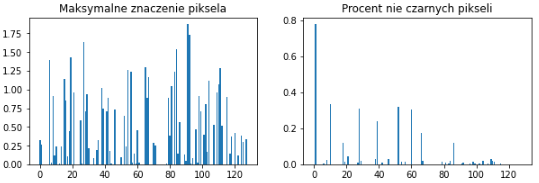
\includegraphics[width=0.8\textwidth,keepaspectratio=true]{statystyka_warstwy_5}
	\caption{Piąta warstwa splotowa. Działa 81 filtry z 128}
	\label{statystyka_warstwy_5}
\end{figure}

%-----------------------------------------------------------------------------------
\section{Eksperymenty}

%-----------------------------------------------------------------------------------
\subsection{Różne struktury sieci}
Pierwszą próbą była sieć zawierająca trzy warstwy splotowe i dwie warstwy "dense". Ta sieć miała w sobie 80,564,612 parametrów. Większą częścią tych parametrów było połączenie ostatniej warstwy splotowej i pierwszej warstwy "dense". To jest bardzo duża liczba parametrów, natomiast średni czas jednej epoki uczenia było 303 sekundy. Ten model osiągną rezultat w val loss: 0.3893 - val accuracy: 0.8630. Co jest całkiem niezły wynik. Na rysunku \ref{history_1} można zobaczyć niewielkie przetrenowanie. 

\begin{figure}[H]
	\centering
	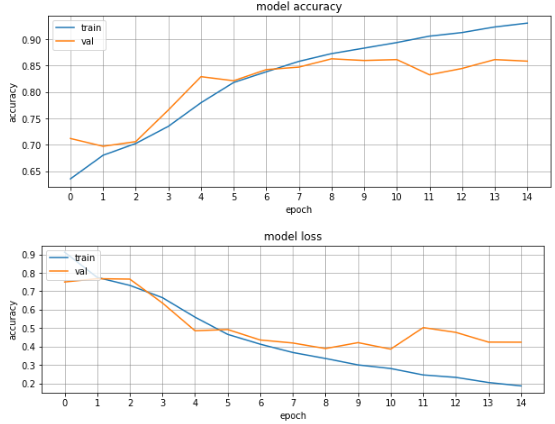
\includegraphics[width=0.8\textwidth,keepaspectratio=true]{history_1}
	\caption{Historia uczenia 1 modeli}
	\label{history_1}
\end{figure}

Drugi model miał łącznie 4,486,116 parametrów i zawierał 4 warstwy splotowe i trzy "dense". W historii uczenia tego modelu (rysunek \ref{history_2}) widać że coś poszło nie tak. Przez ostatnie cztery epoki nie było ulepszeń i uczenie zostało przerwane.

\begin{figure}[H]
	\centering
	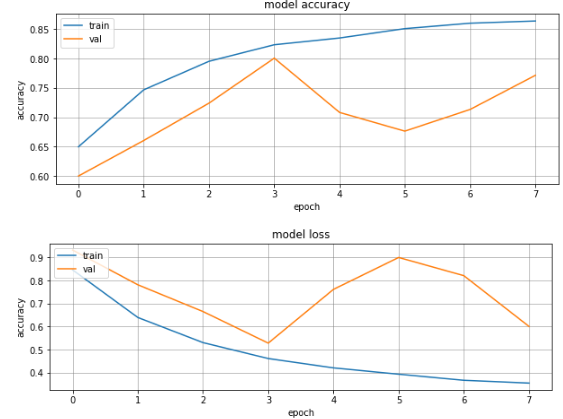
\includegraphics[width=0.8\textwidth,keepaspectratio=true]{history_2}
	\caption{Historia uczenia 2 modeli}
	\label{history_2}
\end{figure}

Trzeci model miał 4 warstwy splotowe i 3 "dense". Liczba parametrów równa się 32,157,444. To nie ulepszyło sytuacje.

\begin{figure}[H]
	\centering
	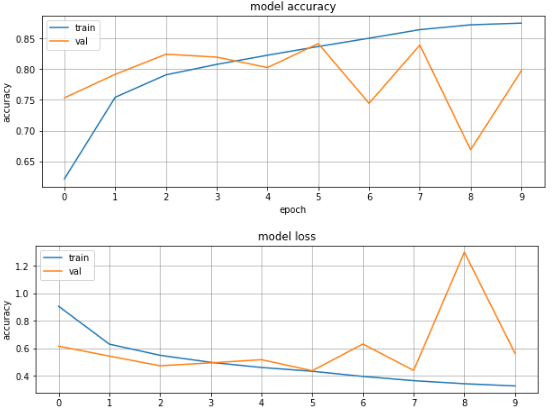
\includegraphics[width=0.8\textwidth,keepaspectratio=true]{history_3}
	\caption{Historia uczenia 3 modeli}
	\label{history_3}
\end{figure}

Czwarty raz spróbowałem wziąć najpierwszy model, dodać jedną warstwe splotowa  BatchNormalization po każdej warstwie splotowej. W teorii to miało by ulepszyć wynik i zwiększysz szybkość uczenia się. Ale niestety ani jedno ani drugie nie było fajne. Prędkość była około 345 sekund na epokę.

\begin{figure}[H]
	\centering
	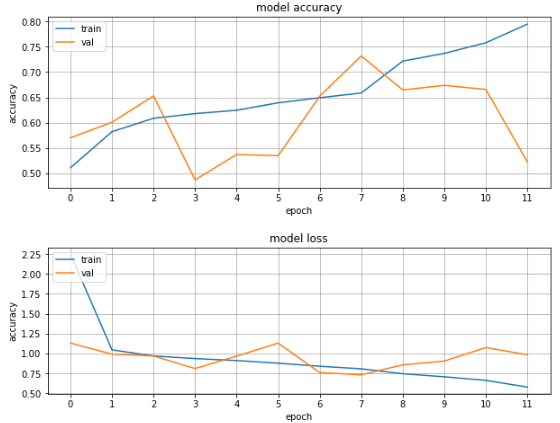
\includegraphics[width=0.8\textwidth,keepaspectratio=true]{history_4}
	\caption{Historia uczenia 4 modeli}
	\label{history_4}
\end{figure}

W piątym modelu kluczową zmianą było to że pierwsze dwie warstwy splotowe idą jedna po drugiej bez żadnej warstwy po środku. I do tego jeszcze rozmiary filtrów splotowych były po kolei 64, 64, 32, 32. Czyli odwrotnie, do tej pory robiłem rosnąco. Widać trochę przetrenowanie na końcu ale nie krytycznie. Liczba parametrów -- 20,203,396. Jest to cztery razy mniej od pierwszego modelu a rezultat jest nie gorszy.

\begin{figure}[H]
	\centering
	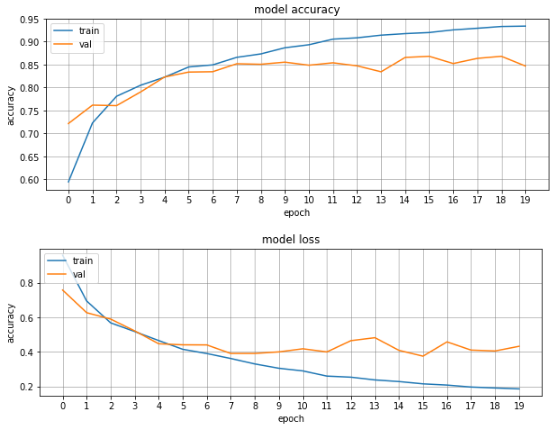
\includegraphics[width=0.8\textwidth,keepaspectratio=true]{history_5}
	\caption{Historia uczenia 5 modeli}
	\label{history_5}
\end{figure}

W szóstym i ostatnim modelu, w odróżnieniu od piątego, dodałem jedną warstwę splotową i rozmiar filtrów jest ustawiony rosnąco. Dodanie warstwy splotowej zmniejszyło wielkość ostatniej mapy cech, co zmniejsza ilość parametrów. W tym modelu jest to 16,983,268. Plus do tego to zwiększyło prędkość uczenia się, 184 sekundy na epokę. Ten model wyszedł najlepszy względem liczby parametrów i prędkością działania i też daje najlepszy rezultat, wprawie 87\% wiarygodności predykcji chorób w zbiorze testowym.  

\begin{figure}[H]
	\centering
	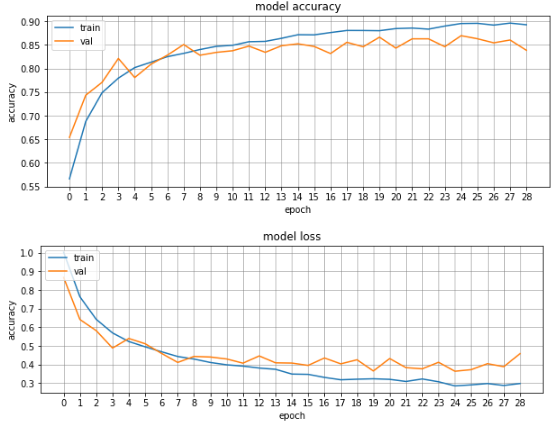
\includegraphics[width=0.8\textwidth,keepaspectratio=true]{history_6}
	\caption{Historia uczenia 6 modeli}
	\label{history_6}
\end{figure}


%-----------------------------------------------------------------------------------
\subsection{Sprawdzenie prawidłowości klasyfikacji}

Na rysunkach niżej próbowałem czy sieć reaguje tylko na płuca i choroby czy inne czynniki (literki, strzałki napisy...) mają wpływ.


\begin{figure}[H]
	\centering
	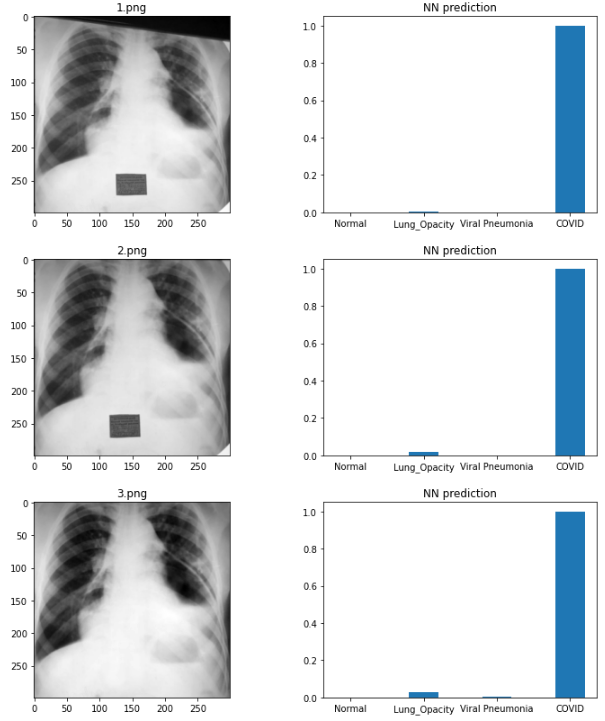
\includegraphics[width=0.8\textwidth,keepaspectratio=true]{fixing_image_exp}
	\caption{W tym przypadku wyrównanie i usunięcie karteczki na dole nie spowodowało żadnych poważnych zmian w predykcji }
	\label{}
\end{figure}

\begin{figure}[H]
	\centering
	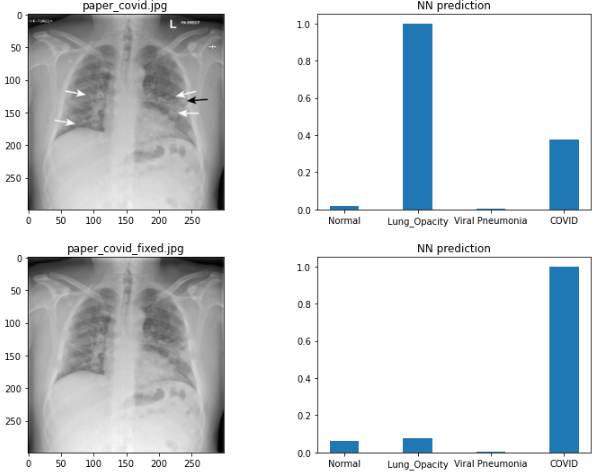
\includegraphics[width=0.8\textwidth,keepaspectratio=true]{paper_covid_exp}
	\caption{Usuniecie strzałek i literki prawym górnym rogu całkowicie zmieniły rezultat predykcji}
	\label{}
\end{figure}

\begin{figure}[H]
	\centering
	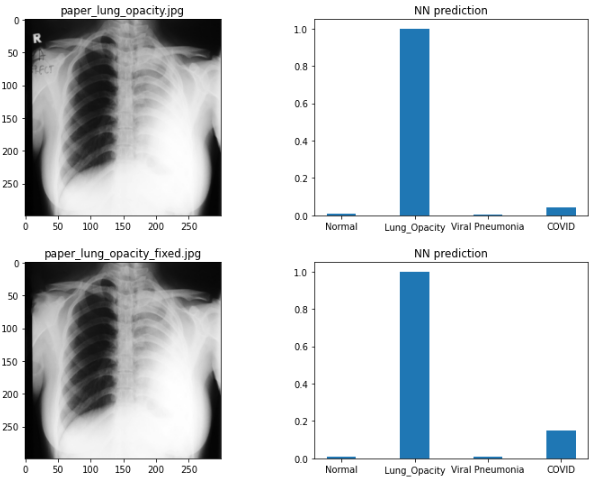
\includegraphics[width=0.8\textwidth,keepaspectratio=true]{paper_l_o_exp}
	\caption{Litera R nie wpływa na predykcje}
	\label{}
\end{figure}

\begin{figure}[H]
	\centering
	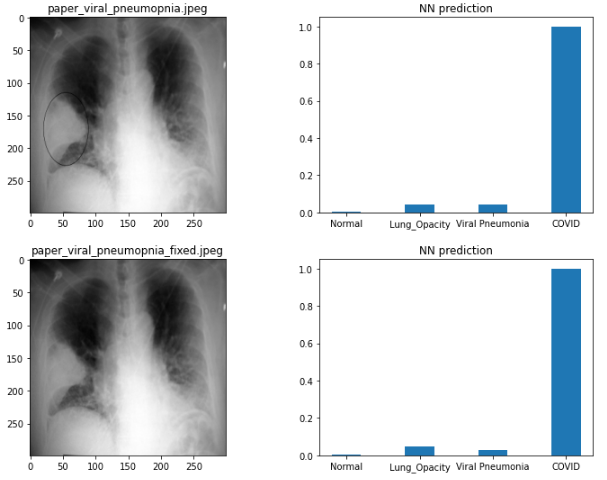
\includegraphics[width=0.8\textwidth,keepaspectratio=true]{paper_v_p_exp}
	\caption{Usuniecie koła nie powoduje zmian}
	\label{}
\end{figure}

\begin{figure}[H]
	\centering
	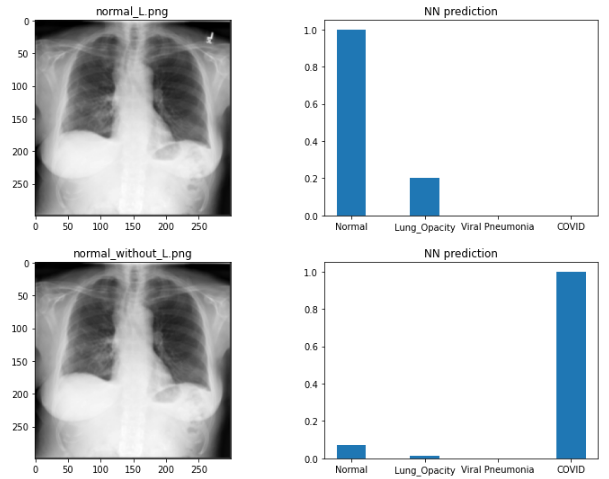
\includegraphics[width=0.8\textwidth,keepaspectratio=true]{normal_L_exp}
	\caption{Tutaj można wyciągnąć wniosek że predykcja zależy od literki w prawym górnym rogu}
	\label{}
\end{figure}

\begin{figure}[H]
	\centering
	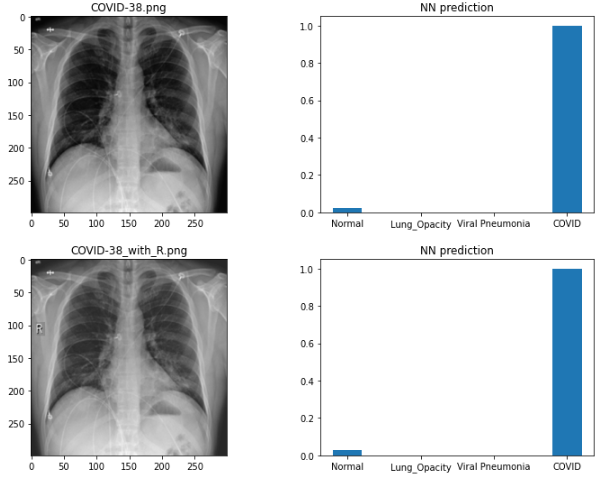
\includegraphics[width=0.8\textwidth,keepaspectratio=true]{covid_R_exp}
	\caption{Dodanie literki R(literka była wzięta ze "zdrowego" zdjęcia nie powoduje zmian)}
	\label{}
\end{figure}

\begin{figure}[H]
	\centering
	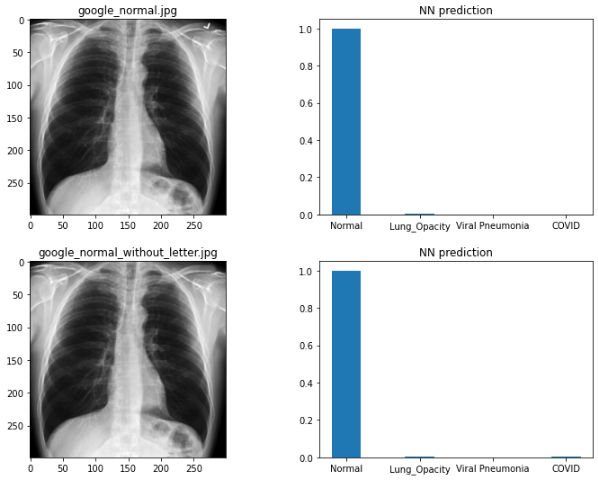
\includegraphics[width=0.8\textwidth,keepaspectratio=true]{google_normal_L_exp}
	\caption{Akurat w tym przypadku litera nie wpływa na rezultat predykcji}
	\label{}
\end{figure}



%-----------------------------------------------------------------------------------
\section{Wnioski}
Rezultat uczenia był zachęcający, w to że prawdopodobieństwo zgadywania chorób 87\% można uwierzyć. Ale jak pokazują eksperymenty i sprawdzanie, sieć czasem generuje odpowiedź na podstawie różnych literek, strzałek znajdujących się na RTG zdjęciu. Natomiast oczekujemy zależność predykcji od zmian płuc w odróżnieniu od zdrowych. To że na zbiorze testowym wynik jest względnie wysoki może wskazywać na złe dane treningowe i testowe. To znaczy że są jakieś zależności ukryte na podstawie których sieć i robi swoją predykcje. Można z tego wyciągnąć wniosek że sieć nauczyła się poprawnie ale dane treningowe są nie wysokiej jakości. Jako pomysł na dalszą pracę w rozwiązywaniu tego problemu można przeprowadzić wstępne przetwarzanie danych. Można by było pododawać różne losowe literki, strzałki i obiekty do zdjęć żeby nie było sensu dla sieci patrzeć na to, żeby te obiekty były szumem. W tedy, teoretycznie, sieć mogła by więcej resursu poświadczyć na znalezienie chorób.

\bibliography{bibliografia}
	
\end{document}